\documentclass[a4paper,11pt]{article}
\usepackage[dvips]{graphicx}
\usepackage{amssymb,amsmath,amsthm}
\newcommand{\dd}{\text{d}}

\usepackage{makeidx}
\makeindex 
\author{Sebastian Bodenstein}
\title{Solutions for Problems in Penrose's The Road to Reality}
\setcounter{secnumdepth}{-1} 
\begin{document}


\maketitle
\tableofcontents

\newpage
\section{5. Geometry of Logarithms, Powers and Roots}
% --------------------------------------
% Chapter 5 Solutions
% --------------------------------------

\subsection{5.5 $\bigstar \bigstar \bigstar$}
Let us first look at $e^a e^b$.
\begin{align*}
e^a e^b&=e^a(1+b+\frac{b^2}{2!}+\ldots)=e^a+e^a b+\frac{e^a b^2}{2!}+\ldots+\frac{e^a b^k}{k!}+\ldots\\
&=\sum^{\infty}_{n=0}\frac{a^n}{n!}+\sum^{\infty}_{n=0}\frac{a^nb}{n!} +\ldots+\sum^{\infty}_{n=0}\frac{a^n b^k}{n! k!}+\ldots\\
&=\sum_{k=0}^{\infty}\left(\sum^{\infty}_{n=0}\frac{a^n b^k}{n! k!}\right)
\end{align*}
Now consider $e^{a+b}$.We are given that the coefficient of $a^p b^q$ in $(a+b)^n$ is $\frac{n!}{p!q!}$. But we know that $p+q=n$. So let $p=n-q$, then  
\begin{equation}
(a+b)^n=\sum^{n}_{k=0}\frac{n!}{k!(n-k)!}a^{n-k}b^k
\end{equation}
Then we have that
\begin{align*}
e^{a+b}=\sum^{\infty}_{n=0}\frac{(a+b)^n}{n!}&=\sum^{\infty}_{n=0}\left(\sum^{n}_{k=0}\frac{1}{k!(n-k)!}a^{n-k}b^k\right)
\end{align*}
To see that this is the same as for $e^ae^b$, let us consider what the above sum means. Suppose we fix $k=i$. This will only exist when $i\leq n$. Then the sum becomes 
$$\sum^{\infty}_{n=i}\frac{1}{i!(n-i)!}a^{n-i}b^i=\sum^{\infty}_{q=0}\frac{1}{i!q!}a^q b^i$$
using $q\equiv n-i$. But the above must be summed over all $k$, not just for $k=i$. And as $n$ has range to $\infty$, so must $k$. So 
\begin{align*}
e^{a+b}=\sum^{\infty}_{n=0}\left(\sum^{n}_{k=0}\frac{1}{k!(n-k)!}a^{n-k}b^k\right)=\sum^{\infty}_{k=0}\sum_{q=0}^{\infty} \frac{1}{k!q!}a^q b^k=e^ae^b
\end{align*}




\newpage
\section{6. Real-number calculus}
% --------------------------------------
% Chapter 6 Solutions
% --------------------------------------

\subsection{6.1 $\bigstar$}
Suppose $x>0$. Then $|x|=x$, and so
$$\theta(x)=\frac{x+x}{2x}=1$$
If $x<0$, then $|x|=-x$, and so
$$\theta(x)=\frac{-x+x}{2x}=0$$


\subsection{6.2 $\bigstar \bigstar \bigstar$}
The technique to prove this is almost identical to that in problem [6.4], which we have worked out in detail.


\subsection{6.3 $\bigstar$}
It seems that the relevant rules are in the beginning of section 6.5, rather than at the end. \\ \\ To show this, we simply differentiate, then set to 0. Then differentiate again and again set to zero, etc. In this way we get each of the coefficients $a_n$. So iff $f(x)=a_0+a_1 x+a_2 x^2+\ldots$ then obviously $f(0)=a_0$. Differentiating once, 
$$\frac{\dd f(x)}{\dd x}=a_1+2a_2 x+3a_3 x^2+\ldots$$
So then $f'(0)=a_1$. To get the $n^{th}$ term, we evidently have to differentiate $n$ times and set to zero.
\begin{align*}\frac{\dd^n f(0)}{\dd x^n}&=n(n-1)(n-2)\ldots 1\cdot a_n+(n+1)\cdot n \cdot(n-1)\ldots 1 a_{n+1}0+ \ldots\\
&=n!a_n
\end{align*}
and so $$a_n=\frac{f^{(n)}(0)}{n!}$$.


\subsection{6.4 $\bigstar \bigstar \bigstar$}
To show that the function 
$$f(x)=e^{-\frac{1}{x^2}}$$
is $C^{\infty}$ we need to show that each of its derivatives is continuous. Iff we differentiate once, we get
$$\frac{\dd f(x)}{\dd x}=\frac{2 e^{-\frac{1}{x^2}}}{x^3}$$
If we differentiate more often, we will see a pattern: each derivative is a sum of terms of the form $A x^{-n} e^{-\frac{1}{x^2}}$ where $A$ is some constant. Indeed
$$\frac{\dd }{\dd x}\left(\frac{e^{-\frac{1}{x^2}}}{x^n}\right)=\frac{2 e^{-\frac{1}{x^2}}}{x^{n+3}}-\frac{n e^{-\frac{1}{x^2}}}{x^{n+1}}$$
So if one derivative is a sum of terms of the form $A x^{-n} e^{-\frac{1}{x^2}}$, then all subsequent derivatives will also be of this form, which is what we claimed. \\ \\ Now iff the term $A x^{-n} e^{-\frac{1}{x^2}}$ is continuous, we note that that finite sums of these terms are also continuous. Let us first show continuouity\footnote{We say a function $f(x)$ is continuous at $x=0$ iff $\lim_{x\to 0} f(x)$ is the same whether the limit goes from above or below.} $x=0$. \\ \\ We see that as $x\to 0^\pm$, $e^{-1/x^2}\to 0$ and $x^{-n}\to \pm \infty$. So does $e^{-1/x^2}$ tend to 0 faster than $x^{-n}$ tends to $\infty$? The answer is yes. To see this, consider the power-series\footnote{We could also use \emph{L'Hospitals Rule} here.} obtained by expanding the exponent: 
\begin{align*}
e^{1/x^2}&=1+\frac{1}{x^2}+\frac{1}{2!\cdot x^4 }+\ldots \frac{1}{(n+1)!\cdot x^{2n+1}}+\ldots  > \frac{1}{(2n+1)!\cdot x^{2n+1}}\\
\implies  \ \ \ \ \ e^{-\frac{1}{x^2}}&< (2n+1)!\cdot x^{2n+1}\\
\implies \ \ \ \ \ \lim_{x\to 0}\frac{e^{-\frac{1}{x^2}}}{x^n}&<\lim_{x\to 0} \frac{(2n+1)!x^{2n+1}}{x^n}=(2n+1)!\lim_{x\to 0} x^{n+1}=0
\end{align*}
The argument above applies regardless of whether the limit is from above or below, and hence every derivative is continuous at $x=0$. It is easy to see that the function is continuous everywhere else, as we know in general that if $I$ and $J$ are intervals, $f:I\to\mathbb{R}$ is continuous at $x\in I$ ($f(x)\in J$) and $g: J\to \mathbb{R}$ is continuous at $f(x)$, then the composition $g\circ f$ is also continuous at $x$. In our case, $f(x)=e^x$ and $g(x)=-x^{-2}$ which are both obviously continuous at $x\neq 0$, and hence the composition of them is also continuous on this domain. Muliplying this with $x^{-n}$ will again yield a continuous function (in the defined domain), as multiplying continuous functions preserves continuouity.  And so we have that $k(x)=A x^{-n} e^{-\frac{1}{x^2}}$ is continous for all $\mathbb{R}$, and hence all the derivatives of $f(x)=e^{-\frac{1}{x^2}}$ are continuous, and hence our function is $C^{\infty}$ smooth. 
\\ \\ Now we need to show that $f(x)=e^{-\frac{1}{x^2}}$ is not analytic at $x=0$. This is easy, as suppose $f(x)$ can be expressed by a power series about $x=0$. Then 
$$f(x)=f(0)+\frac{f'(0)}{1!}x+\frac{f''(0)}{2!}x^2+\frac{f'''(0)}{3!}x+\ldots$$
But we have just shown that each derivative vanishes at $x=0$. So the power-series also vanishes, and tells us that $f(z)=0$, which is nonsense. As there is no power-series representation about $z=0$, it is not analytic there.


\subsection{6.5 $\bigstar$}
We were given previously that $e^x=\sum^{\infty}_{n=0}\frac{x^n}{n!}=1+\sum^{\infty}_{n=1}\frac{x^n}{n!}$. Then
\begin{align*}
\text{d}e^x=\text{d}(1)+\text{d}\sum^{\infty}_{n=1}\frac{x^n}{n!}=0+\sum^{\infty}_{n=1}\frac{nx^{n-1}\text{d}x}{n!}=\sum^{\infty}_{n=1}\frac{x^{n-1}}{(n-1)!}\text{d}x=\sum^{\infty}_{n=0}\frac{x^n}{n!}\text{d}x=e^x\text{d}x
\end{align*}
where we made use of $\frac{n}{n!}=\frac{n}{n\cdot(n-1)\cdot\ldots\cdot 1}=\frac{1}{(n-1)!}$.


\subsection{6.6 $\bigstar \bigstar$}
We will prove this using induction. We first need the obvious fact that $\frac{\text{d}x}{\text{d}x}=1$. The formula $\text{d}(x^n)=nx^{n-1}\text{d}x$ then obviously holds for $n=1$. Now suppose it holds for some $n=k$. Then
\begin{align*}
\frac{\text{d}(x^{k+1})}{\text{d} x}=\frac{\text{d}(x\cdot x^{k})}{\text{d} x}&=\frac{\text{d}x}{\text{d} x}\cdot x^k+x\frac{\text{d}(x^{k})}{\text{d} x}\\
&=1\cdot x^k+x\cdot kx^{k-1}\\
&=(k+1)x^k
\end{align*} 
So iff it holds for $n=k$, it also holds for $n=k+1$. But it holds for $n=1$, and so also for $n=2$, and then also for $n=3$, etc.


\subsection{6.7 $\bigstar$}
We abbreviate $f(x)\equiv f$ etc. Now let $y=[g]^{-1}$. Then 
$$\text{d} y=\frac{\text{d} y}{\text{d} g}\cdot \text{d} g=-g^{-2}\cdot \text{d} g $$
Then using the Leibniz rule on $fy$, we get
\begin{align*}
d(fy)=y\cdot\text{d}f+f\cdot \text{d}y&=\frac{\text{d}f}{g}-\frac{f\cdot \text{d} g}{ g^{2}}\\
&\frac{g\cdot\text{d}f-f\cdot \text{d} g}{ g^{2}}
\end{align*}


\subsection{6.8 $\bigstar$}
Let $y(u(x))=u^4$, where $u=1-x^2$. Then
$$\frac{\text{d} y}{\text{d}x}=\frac{\text{d} y}{\text{d}u}\cdot\frac{\text{d} u}{\text{d}x}=4u^3\cdot (-2x)=-8x(1-x^2)^3$$
Let us look at the other function. Using the `quotient' rule, we quickly get
$$\frac{\text{d} }{\text{d}x}[(x+1)(1-x)^{-1}]=\frac{(1-x)\cdot 1 -(x+1)\cdot (-1)}{(1-x)^2}=\frac{2}{(1-x)^2}$$


\subsection{6.9 $\bigstar\bigstar$}
We will assume all of the results obtained in question [6.10]. \\ \\ Lets do $y=x^x$ first. $\log y=x\log x\implies y^{-1}\dd y=(\log x +1)\dd x$. From this we get
$$\dd(x^x)= x^x(\log x +1)\dd x$$ 
For the second one, let us first work out $\dd \log x$. Let $y=e^x\implies \log y = x$. Then using the `chain-rule', 
\begin{align*}
\dd(\log y)&=y'\cdot (\log y)'\dd x=e^x\cdot (\log y)'\dd x=\dd(x)=\dd x\\
\implies \ \ \ (\log y)'&=\frac{1}{e^x}=\frac{1}{y}
\end{align*}
And now it is obvious to see that
$$\dd(\log_a x)=\frac{\dd x}{x \log a}$$
as $$\log_a x=\frac{\log x}{\log a}$$
For the last one, let $y=x^{\log_x a}=a$. Then $\log y = \log_x a \cdot \log x=\log a \implies \dd(\log y)=x^{-1}\log_x a\,\dd x+\log x\cdot \dd(\log_x a)=0$. From this we get
$$ \dd(\log_x a)=-\frac{\log_x a}{x\cdot \log x}\dd x=-\frac{\log a}{x\cdot (\log x)^2}\dd x$$


\subsection{6.10 $\bigstar\bigstar$}
\begin{itemize}
\item[1.] We know that $e^{\log x}=x$. Then $\text{d}(e^{\log x})=\text{d}(x)\implies e^{\log x}\cdot \text{d}(\log x)=1\implies x \cdot \text{d}(\log x)=1 $ from which the result follows.
\item[2.] We know that $e^{i x}=\cos x +i\sin x$. Then $\text{d}e^{ix}=\text{d}(\cos x) +i\text{d}(\sin x)$. But also $\text{d}e^{ix}=i e^{ix} \text{d}x=(i\cos x -\sin x)\text{d}x$. Now we know that $\text{d}(\cos x)$ and $\text{d}(\sin x)$ are real (slopes of real functions are obviously real numbers) and so $\text{d}(\cos x)$ corresponds to the real part of $\text{d}e^{ix}$, and $\text{d}(\sin x)$ the imaginary part. Hence $\text{d}(\cos x)=-\sin x\,\text{d}x$ and $\text{d}(\sin x)=\cos x \,\text{d}x$. 
\item[3.] $\sin(\sin^{-1}x)=x\implies \cos(\sin^{-1}x)\cdot\dd (\sin^{-1}x)=\dd x\implies \dd (\sin^{-1}x)=\frac{\dd x}{\cos(\sin^{-1}x)}$. Now using \textbf{Fig 1}, we see that $\sin^{-1}x=\theta$. Also, $\cos\theta=y$. We also have that $x^2+y^2=1\implies y=\sqrt{1-x^2}$. Hence $\cos(\sin^{-1}x)=y=\sqrt{1-x^2}$. Putting this together, we have that
$$\dd (\sin^{-1}x)=\frac{\dd x}{\sqrt{1-x^2}}$$
\begin{figure}
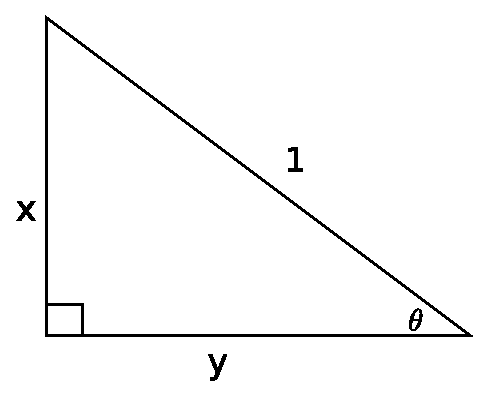
\includegraphics[scale=0.5]{chapters/images/triangle.eps}
\caption{  }
\end{figure} 
\end{itemize}
The remaining expressions are obtained in exactly the same way, and we won't do them here. 





\newpage
\section{7. Complex-number calculus}
% --------------------------------------
% Chapter 7 Solutions
% --------------------------------------


\subsection{7.1 $\bigstar$}
This basically stems from the fact that integrating $z^{n}$ will give $\frac{1}{n+1}z^{n+1}$, when $n\neq -1$. But the function $f(z)=z^{n+1}$ is not multivalued, thus the integral must vanish.\\ \\ To see this explicitly, suppose $z'$ is $z$ rotated by $2\pi$, i.e $z'=z\cdot e^{2i\pi}$. Then $(z')^{(n+1)}=z^{n+1}\cdot e^{2i\pi(n+1)}=z^{n+1}$. Hence
$$\int_{z}^{z'}z^n\, dz=\oint z^n\, dz=\frac{1}{n+1}(z')^{n+1}-\frac{1}{n+1}z^{n+1}=0$$


\subsection*{7.2 $\bigstar$}
It is easy to see once we note that $\oint z^n\, dz=0$ for all $n\neq -1$, which we showed in Question 7.1. \\ \\
The Maclaurin expansion of $f(z)$ is $f(z)=\sum_{k=0}^{\infty}\frac{f^{(k)(0)}}{k!}z^k$. Thus
\begin{align*}
\frac{n!}{2\pi i}\oint \frac{f(z)}{z^{n+1}}\, dz&= \frac{n!}{2\pi i}\oint \frac{\sum_{k=0}^{\infty}\frac{f^{(k)}(0)}{k!}z^k}{z^{n+1}}\, dz\\
&= \frac{n!}{2\pi i}\sum_{k=0}^{\infty}\frac{f^{(k)}(0)}{k!}\oint z^{k-n-1}\, dz\\
&=0+0+\ldots +\frac{f^{(n)}(0)}{2\pi i}\oint z^{-1}\, dz+0+0+\ldots\\
&=\frac{f^{(n)}(0)}{2\pi i}\cdot 2\pi i\\
&=f^{(n)}(0)
\end{align*}


\subsection{7.4 $\bigstar\bigstar$}
We will consider the case with 3 poles. First, we note that we can always deform the contour so that we can have closed contours around each of the poles. Each circle contains only one pole. Hence the total integral will be the sum of each of the closed circle integrals.\\ \\
Now we need to evaluate the circular integrals. So let us consider the circle around the pole $a_1$. We have that $h(z)$ is analytic within the contour, hence we can express it as a Taylor series about $a_1$, i.e  $h(z)=\sum_{k=0}^{\infty}\frac{h^{(k)}(a_1)}{k!}(z-a_1)^k$
Thus 
\begin{align*}
f(z)&=\frac{1}{(z-a_1)^n}\sum_{k=0}^{\infty}\frac{h^{(k)}(a_1)}{k!}(z-a_1)^k=\sum_{k=0}^{\infty}\frac{h^{(k)}(a_1)}{k!}(z-a_1)^{k-n}
\end{align*}
Now we have from question [7.1] that $\oint z^n\, dz=0$ for all $n\neq -1$. It is easy to see that the same must be true for $(z+p)^n$. So the closed-integral of $(z-a_1)^{k-n}$ is only non-zero for $k-n=-1 \implies k=n-1$. Thus 
\begin{align*}
\oint_{\gamma_1} f(z)\ dz&=\oint_{\gamma_1} \sum_{k=0}^{\infty}\frac{h^{(k)}(a_1)}{k!}(z-a_1)^{k-n}\ dz\\
&=\sum_{k=0}^{\infty}\frac{h^{(k)}(a_1)}{k!}\oint_{\gamma_1} (z-a_1)^{k-n}\ dz\\
&=\frac{h^{(n-1)}(a_1)}{(n-1)!}\oint_{\gamma_1} (z-a_1)^{-1}\ dz\\
&=\text{Res}[f(z),a_1]\cdot 2\pi i
\end{align*}
as we are given that $\frac{h^{(n-1)}(a_1)}{(n-1)!}=\text{Res}[f(z),a_1]$. Thus the total integral is (the sum of the residues at the poles)$\times 2\pi i$.


\subsection{7.5 $\bigstar\bigstar\bigstar$}
\textbf{Question:} \ Show that
$$\int^{\infty}_{0}x^{-1}\sin x=\frac{\pi}{2}$$
\textbf{Strategy:} Penrose recommends we consider the function $f(z)=z^{-1} e^{iz}$ instead of the obvious $z^{-1} \sin z$.\footnote{The reason for this is that the integral of $z^{-1} \sin z$ around the semicircle $\Gamma_1$ does not go to 0 as $R\to\infty$. It is much easier showing things go to zero than explicity evaluating them, and so we avoid this difficulty by integrating around $z^{-1} e^{iz}$ instead.}   We integrate along the contour in \textbf{Fig. 1}. We can easily find the value of the total integral using the Cauchy formula, $\oint f(z)z^{-1}\, \text{d}z=2\pi i\cdot f(0)$ (Road TR pg 127). We can then calculate the contribution from $\Gamma_2$ as $\epsilon\to 0$, and we will show that as $R\to \infty$, $\Gamma_1\to 0$. Then the contribution from the real axis plus $\Gamma_2$ equals what we got using the Caucy formula. Thus we can get the value of the integral along the real axis. Finally, we know that the original integral is just the imaginary part of the integral of $z^{-1} e^{iz}$.\\ \\
\begin{figure}\label{e}
\includegraphics[scale=0.8]{chapters/images/7.5.eps}
\caption{The contour along which we integrate $f(z)=z^{-1} e^{iz}$, with the star indicating the singularity at the origin.  }
\end{figure}  
\textbf{Solution:} Making use of the Cauchy formula, and that in general $z=x+iy$ so $z=x$ on the real-axis,
\begin{align*}
\oint_\Gamma z^{-1}e^{iz} \ dz &= 2\pi i e^{i\cdot 0}=2\pi i\\
&=\int_{\Gamma_1} z^{-1}e^{iz}\ dz+\int_{\Gamma_2} z^{-1}e^{iz}\ dz+\int_{-R}^{-\epsilon} x^{-1}e^{ix}\ dx+\int^{R}_{\epsilon} x^{-1}e^{ix}\ dx
\end{align*}
It turns out that 
$$\lim_{R\to \infty}\int_{\Gamma_1} z^{-1}e^{iz}\ dz =0$$
This is difficult to show directly. It is easiest making use of a result not given in the Road TR, known as \emph{Jordan's lemma}. The statement (and simple proof) of the Lemma is given in the Appendix, from which it is easy to see that this result follows.\footnote{This may seem as cheating, but the method of the proof could be used to directly get the result. Why not just get the general result instead?} \\ \\
Now we want to find the value of the integral along $\Gamma_2$ as $\epsilon\to 0$. We give two different ways of getting this.
\subsection*{Evaluating $\Gamma_2$, method 1}
\begin{align*}
\lim_{\epsilon \to 0} \int_{\Gamma_2} z^{-1}e^{iz}\, dz&=\lim_{\epsilon \to 0} \int_{\Gamma_2} z^{-1}\left[ 1+\frac{1}{1!}(iz)+\frac{1}{2!}(iz)^2+\ldots\right ]dz\\
&=\lim_{\epsilon \to 0} \int_{\Gamma_2} z^{-1}\ dz+\lim_{\epsilon \to 0} i\int_{\Gamma_2} dz-\lim_{\epsilon \to 0} \frac{1}{2}\int_{\Gamma_2} z \ dz+\ldots
\end{align*} 
But $\lim_{\epsilon \to 0} \int_{\Gamma_2} z^{n}\ dz=0$
for all $n\geq 0$.\footnote{The maximum value of $z^n$ on $\Gamma_2$ goes to 0 as $\epsilon \to 0$, and the length of  $\Gamma_2$ also goes to zero. Hence the integral must also go to zero.} Hence 
$$ \lim_{\epsilon \to 0} \int_{\Gamma_2} z^{-1}e^{iz}\, dz=\lim_{\epsilon \to 0} \int_{\Gamma_2} z^{-1}\ dz$$
 Now we know that $z=\epsilon e^{i\phi}$. Hence 
$$d z=i \epsilon e^{i\phi}d\phi$$
Thus 
\begin{align*}
\lim_{\epsilon \to 0} \int_{\Gamma_2} z^{-1}\ dz&=\lim_{\epsilon \to 0} \int^{0}_{-\pi} \frac{1}{\epsilon e^{i\phi}}i \epsilon e^{i\phi}d\phi \\
&=i\lim_{\epsilon \to 0} \int^{0}_{-\pi} d\phi =i\pi \\
\end{align*}
\subsection*{Evaluating $\Gamma_2$, method 2}
The result can be obtained using only Cauchy's formula, and symmetry. We do this here. So using Eulers formula, we have that 
\begin{align*}
 \int_{\Gamma_2} z^{-1}e^{iz}\, dz&= \int_{\Gamma_2} z^{-1}\cos z\, dz+i \int_{\Gamma_2} z^{-1}\sin z\, dz
\end{align*}
Now suppose we chose to integrate around a complete circle centred on $z=0$. In this case, we can use Cauchy's formula:
\begin{align*}
 \oint z^{-1}\cos z\, dz+i \oint z^{-1}\sin z\, dz&=2\pi i \cos(0)+2\pi i \cdot i \sin (0)\\
&=2 \pi i+0
\end{align*}
The circle consists of two semicircles, $\Gamma_2$ and, let us call the other $\phi$. Now $\Gamma_2$ is evaluated from $z=-\epsilon$ to $z=\epsilon$, then let $\phi$ be evaluated from $z=\epsilon$ to $z=-\epsilon$. Now as $f(z)=z^{-1}\sin z$ is a symmetric, i.e $f(-z)=f(z)$, we have that $$\int_{\Gamma_2} z^{-1}\sin z\, dz= \int_{\phi} z^{-1}\sin z\, dz$$
Hence 
$$\oint z^{-1}\sin z\, dz=\int_{\Gamma_2} z^{-1}\sin z\, dz+ \int_{\phi} z^{-1}\sin z\, dz=2 \int_{\Gamma_2} z^{-1}\sin z\, dz=0$$
Next, we note that $z^{-1}\cos z$ is antisymmetric, and hence 
$$\int_{\Gamma_2} z^{-1}\cos z\, dz=- \int_{\phi} z^{-1}\cos z\, dz$$ 
Hence $\int_{\Gamma_2} z^{-1}\cos z\, dz=\pi i$ and so $\int_{\Gamma_2} z^{-1}e^{iz} \, dz=\pi i$.\\ \\
Putting the contributions to all the paths together, and noting that
$$\int_{-R}^{-\epsilon} x^{-1}e^{ix}\ dx=\int^{R}_{\epsilon} x^{-1}e^{ix}\ dx,$$
we get that
\begin{align*}
\oint_\Gamma z^{-1}e^{iz} \ dz &=2i\pi \\
&=0+i\pi+2\lim_{\frac{1}{R},\epsilon\to 0}\int^{R}_{\epsilon} x^{-1}e^{ix}\ dx\\
&=i\pi+2\int^{\infty}_{0} x^{-1}e^{ix}\ dx\\
\implies  \ \ \ \ \ \ \ &\int^{\infty}_{0} x^{-1}e^{ix}\ dx =i\frac{\pi}{2} \\
\implies  \ \ \ \ \ \ \ &\int^{\infty}_{0} x^{-1}\cos x\ dx+i\int^{\infty}_{0} x^{-1}\sin x\ dx =i\frac{\pi}{2}
\end{align*}
This implies that $\int^{\infty}_{0} x^{-1}\cos x\ dx=0$, as it is real and the real part of $i\frac{\pi}{2}$ is 0. Hence
$$\int^{\infty}_{0} x^{-1}\sin x\ dx =\frac{\pi}{2}$$


\subsection{7.6 $\bigstar\bigstar \bigstar$}
Let $$f(z)=z^{-2}\cot z\pi=z^{-2}\cos z\pi(\sin z\pi)^{-1}$$
We integrate about the square contour $\Gamma$ as shown in \textbf{Fig. 2}. We know from question [7.4] that this integral will equal the sum of the residues within the contour. Hence
\begin{equation}\label{totalint}
\frac{1}{2\pi i}\oint_\Gamma f(z)=\text{Res}[f(z),0]+\sum^{-1}_{n=-N}\text{Res}[f(z),n]+\sum^{N}_{n=1}\text{Res}[f(z),n]\end{equation}
Let us investigate the residues. The function $f(z)$ has a pole at $z=0$ and whenever $\sin \pi z=0$, which will be when $z=n$, $n\in \mathbb{Z}$. Penrose recommends that we use the results of [7.4]. In order to use the formula for the residue, we need to know what order pole we dealing with. At $z=0$, $(\sin \pi z)^{-1}$ has a pole of order 1 also. One can easily see this from the series $(\sin \pi z)^{-1}=(\pi z-\frac{(\pi z)^3}{3!}+\ldots)^{-1}=(\pi z)^{-1}(1-\frac{(\pi z)^2}{3!}+\ldots)^{-1}=(\pi z)^{-1} g(z)$, where $g(z)$ is obviously regular at $z=0$. As $\cos \pi z= 1+\ldots$, we have that the pole of $f(z)$ at $z=3$ is of order 3. The other poles at $z=n$, $n\neq 0$ are obviously of order 1.\footnote{This is not obvious from the series, but due to the periodicity of $\sin z$, if the pole at $z=0$ is order 1, then the others must be too. This is because $\sin(\pi n)=\pm \sin(0)$ (depending on $n$ even or odd), so has order 1.}\\ \\
Lets find the residue at $z=0$. To do this, first note that we can write $f(z)=z^{-3}h(z)$ where $h(z)=z\cot \pi z$, and is regular around $z=0$. Also,\footnote{This is easy to find using the Quotient rule on pg. 115 RTR, and won't bother showing it here.}
$\frac{d }{d z}\cot \pi z=\frac{\pi}{\sin^2(\pi z)}=\pi \csc^2(\pi z)$
Then from [7.4], we have that 
\begin{align*}
\text{Res}[f(z),0]&=\lim_{z\to 0}\left[\frac{1}{2!}\frac{d^2 h(z)}{d z^2}\right]=\lim_{z\to 0}\left[2\pi^2 z \cos(\pi z) \csc^3(\pi z)-2\pi\csc^2(\pi z)\right]\\
&=\lim_{z\to 0}\left[  \pi^2 z \cos(\pi z) -\pi\sin(\pi z)            \right]\csc^3(\pi z)\\
&=\lim_{z\to 0}\pi\cdot\left[ \pi z(1-\frac{(\pi z)^2}{2!}+\ldots)-(\pi z -\frac{(\pi z)^3}{3!}+\ldots)\right]\frac{1}{(\pi z)^3}\cdot \frac{1}{(1+\ldots)^{3}}\\
&=\lim_{z\to 0}\pi\cdot\left[-\frac{(\pi z)^3}{3}+\ldots\right]\frac{1}{(\pi z)^3}\cdot \frac{1}{(1+\ldots)^{3}}\\
&=-\frac{\pi}{3}
\end{align*}
Now we find the residue at $z=n$, $n\neq 0$. As the pole is of order 1, we can write $f(z)=(z-n)^{-1}k(z)$ where $k(z)=z^{-2}(z-n)\cot \pi z$ is regular around $z=n$. Then 
\begin{align*}
\text{Res}[f(z),n]&=\lim_{z\to n} \frac{k(z)}{0!}=n^{-2}\lim_{x\to 0}x\cdot\cot \pi(x+n) \\
&=n^{-2}\lim_{x\to 0}x\cdot\cot \pi x \\
&=n^{-2}\lim_{x\to 0}\frac{x}{\sin \pi x}\\
&=\frac{1}{\pi n^2}
\end{align*}
where we used $x=z-n$, and the last limit was evaluated using the same argument as used previously for $z=0$. We also used the fact that $\cot(x+\pi n)=\cot x$.\\ \\
Putting all this into \eqref{totalint}, we get
\begin{equation}\label{doubletrouble}
\frac{1}{2 i}\oint_\Gamma f(z)\, dz=-\frac{\pi^2}{3}+\sum^{-1}_{n=-N}\frac{1}{ n^2}+\sum^{N}_{n=1}\frac{1}{ n^2}\end{equation}
We can simplify the above by noting that $\sum^{-1}_{n=-N}n^{-2}=\sum^{N}_{n=1}n^{-2}$.\\ \\ We now show that the total integral vanishes when $N\to\infty$.\footnote{We are working towards an answer (that $1+\frac{1}{2^2}+\frac{1}{3^2}+\ldots=\frac{\pi^2}{6}$), and we can easily see from the above equation that for this answer to be correct, the integral must vanish! Not that for some editions of the book, there is a typo, with Penrose telling us the sum equals $\frac{\pi}{6}$ instead of $\frac{\pi^2}{6}$. } We will make use of the fact that 
$$\left|\oint_\Gamma f(z)\, dz\right|\leq L\cdot \text{max}(|f(\Gamma)|)$$
where $L$ is the length of the contour $\Gamma$.\footnote{This is not given by Penrose, but is pretty obvious.} If $L\cdot \text{max}(|f(\Gamma)|)\to 0$ as $N\to\infty$, then the integral must vanish. Now the length of the square-contour is simple $L=4\cdot (2N+1)=8N+4$. \\
We have $|f(z)|=|z^{-2}\cot \pi z|=|z^{-2}|\cdot|\cot \pi z|$. Obviously $|z|>N$, and so $|z^{-2}|<N^{-2}$. Let us look at the $\cot\pi z$ term. 
\begin{equation*}
|\cot \pi z|=\left|\frac{e^{i\pi z}+e^{-i\pi z}}{e^{i\pi z}-e^{-i\pi z}}\right|=\left|\frac{1+e^{-2i\pi z}}{1-e^{-2i\pi z}}\right|
\end{equation*}
For the vertical sides of the square, $z=\pm(N+0.5)+iy$. For this side, and making use of $e^{\pm 2i\pi(N+0.5)}=-1$,
\begin{align*}
|\cot \pi z|=\left|\frac{1+e^{-2i\pi(\pm N\pm 0.5+iy) }}{1-e^{-2i\pi (N+0.5+iy)}}\right|&=\left|\frac{1-e^{2\pi y}}{1+e^{2\pi y}}\right|\\
&=\left|1-\frac{2}{1+e^{2\pi y}}\right|\leq 1
\end{align*}
For the horizontal sides, $z=x+iy$ with $y=\pm N+0.5$. Using\footnote{These inequalities follow very simply from the geometry of complex numbers.} $\text{max}(|z|,|a|)-\text{min}(|z|,|a|)=\left| |z|-|a|\right|\leq |z+a|\leq |z|+|a|$ and that $|e^{-2i\pi z}|=e^{2\pi y}$,
\begin{align*}
|\cot \pi z|=\frac{|1|+|e^{-2i\pi z}|}{\left| |1|-|e^{-2i\pi z}|\right|}&=\frac{1+e^{2\pi y}}{\left| 1-e^{2\pi y }\right|}\\
&\leq\left|1+\frac{2}{ e^{2\pi y }-1}\right|
\end{align*}
For large $y$, this above tends to $1$, and diverges only for $y=0$. Hence we can find some $k\in \mathbb{R}$, such that for any $N$, $|\cot \pi z|\leq \left|1+2( e^{2\pi y }-1)^{-1}\right|\leq k$
\begin{align*}
\lim_{N\to\infty}\left|\oint_\Gamma z^{-2}\cot\pi z\, dz\right|\leq \lim_{N\to\infty}(8N+4)\cdot |N^{-2}|\cdot k=0
\end{align*}
Hence the integral vanishes as $N\to \infty$. Thus, from \eqref{doubletrouble} we have
\begin{align*}
0&=-\frac{\pi^2}{3}+2\sum^{N}_{n=1}\frac{1}{ n^2}\\
\implies  \ \ \ \ \ \sum^{N}_{n=1}\frac{1}{ n^2}&=\frac{\pi^2}{6}
\end{align*}


\subsection{7.7 $\bigstar\bigstar$}
One way is by recognising $1/z$ to be an incipient geometric series.\footnote{This is not in Road TR, though common maths knowledge. A geometric series is of the form $a+ax+ax^2+\ldots=\frac{a}{1-x}$, where $|x|<1$} So a little manipulation:
\begin{align*}
\frac{1}{z}= -\frac{1}{-p-(z-p)}&=\frac{1/p}{1-(-\frac{z}{p}+1)}\\
&=\sum_{n=0}^{\infty}p^{-1}(-\frac{z}{p}+1)^n\\
&=\sum_{n=0}^{\infty}(-1)^n p^{-(n+1)}(z-p)^n\\
\end{align*}


\subsection{7.8 $\bigstar$}
For a given frequency $n\omega$, we have two contributing exponentials 
\begin{align*}
\alpha_{-n} e^{-in \omega}+\alpha_n e^{in \omega}&=\alpha_{-n}[\cos (-n\omega)+i\sin (-n\omega)]+\alpha_n[\cos (n\omega)+i\sin (n\omega)]\\
&=(\alpha_{-n}+\alpha_n)\cos (n\omega)+i(\alpha_{-n}-\alpha_n)\sin (n\omega)\\
&=a_n\cos (n\omega)+b_n\sin (n\omega)
\end{align*} 
where we made use of $\cos(-x)=\cos x$ and $\sin (-x)=-\sin x$.









\newpage
\section{8. Riemann surfaces and complex mappings}
% --------------------------------------
% Chapter 8 Solutions
% --------------------------------------


\subsection{8.1 $\bigstar$}
We can always write $z=re^{i\theta+2\pi i k}$, where $k$ is some integer. Then $f(z)=z^a=r^a e^{i\theta a+2\pi i ka}$. For 0 turns, $k=0$ and $z^a=r^a e^{i\theta a}$. The Riemann sheets will join together when $2\pi i ka=2\pi i p$, where $p$ is some integer.\footnote{The sheets meet up when $f(z)$ after 0 turns is equal to $f(z)$ after $k$ turns.} This implies that $ka=p\implies a=p/k$. Now suppose $a$ is irrational. By definition, there are no integers $p$ and $k$ such that $a=p/k$. Hence the spiralling sheets will not join again for any number of turns.  \\ \\  
If $a$ is rational, i.e. of form, $a=m/n$ (remembering that $m$ and $n$ have no common factors) then $m/n=p/k\implies p=mk/n$. This equation is first satisfied when $k=n$, and so the sheets meet up after $n$ turns.


\subsection{8.4 $\bigstar \bigstar (\bigstar)$}
This problem is a great deal harder than what Penrose has rated it. It is likely that he made a mistake with the phrasing of the question, and instead meant one had to show that the mapping preserves origin-centred circles, which is much easier.\footnote{I have checked the official correction page for Road to Reality, and there is no correction listed. Perhaps there is an easier way than I know of!}  Indeed, such a circle is given $C=Re^{i\theta}$ where $0\leq\theta<2\pi$. Then if $f(z)=z^{-1}$, then $f(C)=R^{-1}e^{-i\theta}$ which is evidently another origin-centred circle of radius $\tilde{R}=R^{-1}$ and of opposite orientation.\\ \\ 
However, we also want to show the general case. We give here two proofs. The first is the most elegant, but the second is perhaps more direct, and is nice and geometrical.

\subsubsection*{Proof 1: Apollonius}
We use an ancient theorem, due to Apollonius, which gives a useful representation of an arbitrary circle. It states:\\ \\ \emph{Let $t$ be some positive real number. Let $a,b$ be arbitrary complex numbers such that $a\neq b$. Then the locus of points satisfying }
$$|z-a|=t|z-b|$$
\emph{is a circle with radius $R$ and centre $C$, where}
$$R=\frac{t|a-b|}{|t^2-1|} \ \ \ \ \ \ \ \ \ \ C=\frac{t^2 b -a}{t^2-1}$$
Now for a circle centred at $C\neq 0$ of radius $R$, we obviously have that $|z-C|=R$. Now if we apply the transformation $f(z)=z^{-1}$, we have that every point $z \to z^{-1}$, so 
\begin{align*}
|z-C|=R\to |z^{-1}-C|=R&\implies \frac{|z|}{|C|}\left|z^{-1}-C\right|=R\cdot \frac{|z|}{|C|}\\
&\implies\left|z-\frac{1}{C}\right|=\frac{R|z|}{|C|}
\end{align*}
But this is exactly the form of the theorem of Apollonius, and so the inversion of the circle is another circle. Now the observant reader will notice two special cases, when $C=0$ and when $|C|=R$. The case $C=0$ is trivial to show the preservation of the circle. Now when $|C|=R$, we have that $t=1$ in the theorem, and then the radius of the resulting circle is infinite, and the origin of the circle is at infinity. As Penrose mentions somewhere, such a circle is just an infinitely long straight line.

\subsubsection*{Proof 2: Geometry}

 We can parametrize an arbitrary circle centred at $k\in\mathbb{C}$, as $C=Re^{i\theta}+k$ with $0\leq \theta<2\pi$. One strategy to show this is to do as we did for the origin-centred case, and show that 
$$\frac{1}{Re^{i\theta}+k}=\tilde{R}e^{i\tilde{\theta}}+\tilde{k}$$
\begin{figure}[h!]
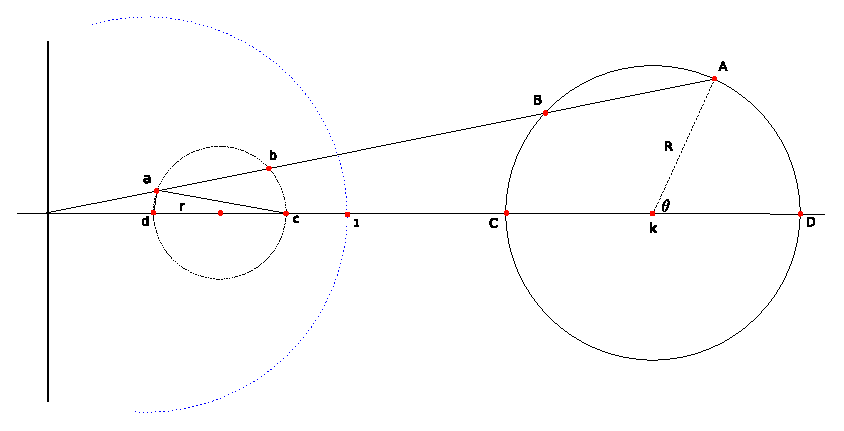
\includegraphics[scale=1.2]{chapters/images/inversion.eps}
\caption{The geometry of the inversion of a circle. }
\end{figure}  

where $\tilde{R}\in\mathbb{R}$, $\tilde{k}\in\mathbb{C}$, and obviously both have no $\tilde{\theta}$ dependance. This can be tried, but quickly one suffocates in the algebra!\footnote{There may an elegant way to do this algebra, but I haven't found it, and not for want of trying!}\\ \\
Lets try a different tactic. We first note that the function $f(z)=z^{-1}=R^{-1}e^{-i\theta}$ can obviously be decomposed into first reflecting all the points about the real-axis, and then inverting the radius. The reflection obviously preserves circles. So lets show that the inversion also does. \\ \\
Consider \textbf{Fig 2}. The big circle is inverted, and we have that $[a]=[A]^{-1}$, $[b]=[B]^{-1}$ etc. Here $[a]$ denotes the magnitude of $[a]$, or distance of $a$ from the origin. The strategy will be to show that the angle $\angle c\hat{a} d=90^{\circ}$. As $A$ is an arbitrary point on the big circle, $a$ will be an arbitrary point on the shape resulting from the inversion of the big circle. But iff for fixed $d$,$c$ every $a$ produces $\angle c\hat{a} d=90^{\circ}$, then we know from circle geometry that $a$ lies on a circle of diameter $[cd]=|[c]-[d]|$.\footnote{The reason for the absoloute magnitude is that we want to keep things general. If the origin was contained within the original circle, then $[c]-[d]$ will be negative.} To show this, we will show that the Pythogarean theorem holds $[ac]^2+[ad]^2=[cd]^2$ for any $a$. But the Pythogarean Theorem only holds iff and only iff $\angle c\hat{a} d=90^{\circ}$.\footnote{The implication $\angle c\hat{a} d=90^{\circ}\implies [ac]^2+[ad]^2=[cd]^2$ is was stated in the beggining of Chapter 2. It is easy to see that the converse $\angle c\hat{a} d=90^{\circ}\implies [ac]^2+[ad]^2=[cd]^2$ must also be true. For suppose $\angle c\hat{a} d=90^\circ$, then $[ac]^2+[ad]^2=[cd]^2$. But suppose I fix the side-lengths $[ac]$ and $[ad]$. Now increasing/decreasing the angle $\angle c\hat{a} d$ will necessarily increase/decrease the hypotenuse $[cd]$. And so any increase/decrease in the angle will break the relation $[ac]^2+[ad]^2=[cd]^2$. So iff the relation holds, the angle must be exactly $90^\circ$.   }   \\ \\
To begin with, suppose we form a triangle between two arbitrary points $a,d$ and the origin $O$. We then have that $[a][A]=1=[d][D]$ from $[A]=a^{-1}$ and $[D]=d^{-1}$.  Then $[a]=([d][A]^{-1})[D]=k [D]$ and $[d]=([a][D]^{-1})[A]=k [A]$ as $k=[d][A]^{-1}=[a][D]^{-1}$. So the triangles $aOd$ and $DOA$ are similar, as the angle $\angle a\hat{O}d=\angle D\hat{O}a$ and the two sides are equal up to a common scale factor. Hence the third side of the two triangles is also related by this scale factor. 
$$[ad]=k[AD]=\frac{[d]}{[A]}[AD]=\frac{[AD]}{[A][D]}$$   
Note that we proved this for arbitrary points, not just the $a$ and $d$ shown in \textbf{Fig 2}. Another simple result we will need (from \textbf{Fig 2}) is that $[AC]^2+[AD]^2=(D-C)^2=4R^2$ as $\angle C\hat{A} D=90^\circ$. \\ \\
We can now state our condition which we wish to show
\begin{align*}
[ad]^2+[ac]^2&=(c-d)^2\\
\implies\ \ \ \ \ \frac{[AD]^2}{[A]^2[D]^2}+\frac{[AC]^2}{[A]^2[C]^2}&=\left(\frac{1}{[D]}-\frac{1}{[C]}\right)^2\\
\implies\ \ \ \ \ [C]^2[AD]^2+[D]^2[AC]^2&=[A]^2\left([D]^2+[C]^2-2[C][D]\right)\\
&=4[A]^2R^2
\end{align*} 
Now we need to show that both sides are equal. We can now use coordinates and just churn out the result.\footnote{Some may be worried that I am only dealing with a very particular circumstance, with the original circle centred on the x-axis. But the inversion does not depend on any angle, it has rotational symmetry. So we can always rotate our coordinates so that this is the case.} It can easily be seen that the following are true:
\begin{align*}
[AD]&=2R\sin(\frac{1}{2}\theta) \\
[AC]&=2R\cos(\frac{1}{2}\theta) \\
[A]^2&=R^2\sin^2\theta+(k+R\cos\theta)^2=R^2+k^2+2kR\cos\theta\\
[C]&=k-R \\
[D]&=k+R
\end{align*}
The right-hand side (RHS) becomes
\begin{align*}
[C]^2[AD]^2+[D]^2[AC]^2&=(k-R)^2[2R\sin(\frac{1}{2}\theta)]^2+(k+R)^2[2R\cos(\frac{1}{2}\theta)]^2\\
&=4k^2R^2+4R^4+8kR^3(\cos^2(\frac{1}{2}\theta)- \sin^2(\frac{1}{2}\theta))\\
&=4R^2(k^2+R^2+2kR \cos\theta)
\end{align*}
where in the last line we made use of the identity $\cos(2\theta)=\cos^2\theta-\sin^2\theta$. Now the left-hand side:
\begin{align*}
4[A]^2R^2&=4\cdot(R^2+k^2+2kR\cos\theta)\cdot R^2\\
&=4R^2(R^2+k^2+2kR\cos\theta)
\end{align*}
which is the same as the RHS. Hence the Pythogorean identity holds, and $\angle c\hat{a} d=90^{\circ}$, and hence the image of the inversion of a circle is another circle. We note also that the argument used was completely general. It did not depend on where the original circle actually was.\footnote{The method used was inspired by the one used by Needham \cite{need}, but with major modifications. He used a beautifully simple argument using the similar triangle property, but one had to consider seperately the case where the origin is contained in the original circle, and a few other considerations were needed to take care of the case where the original circle overlaps the unit circle.}  







\newpage
\section{9. Fourier Decomposition and hyperfunctions}
% --------------------------------------
% Chapter 9 Solutions
% --------------------------------------

\subsection{9.1 $\bigstar$}
For a given frequency $n\omega$, we have two contributing exponentials 
\begin{align*}
\alpha_{-n} e^{-in \omega}+\alpha_n e^{in \omega}&=\alpha_{-n}[\cos (-n\omega)+i\sin (-n\omega)]+\alpha_n[\cos (n\omega)+i\sin (n\omega)]\\
&=(\alpha_{-n}+\alpha_n)\cos (n\omega)+i(\alpha_{-n}-\alpha_n)\sin (n\omega)\\
&=a_n\cos (n\omega)+b_n\sin (n\omega)
\end{align*} 
where we made use of $\cos(-x)=\cos x$ and $\sin (-x)=-\sin x$.


\subsection{9.2 $\bigstar \bigstar$}
We learnt on pg.126 that only the $z^{-1}$ term contributes to the integral \footnote{ie. $\oint z^{-1}\,\rm{d}z=2\pi i$ and that $\oint z^{n}\,\rm{d}z=0$ for all $n\neq -1$.} and hence, taking a contour\footnote{obviously the contour will be contained within the unit circle, as this is the region of analyticity of $F(z)$.} about $z=0$, we get
\begin{align*}
\oint z^{-n-1} F(z)\, \text{d}z&=\oint \frac{1}{z^{n+1}} \left (\ldots +\alpha_{n-1}z^{n-1}+\alpha_{n}z^{n}+\alpha_{n+1}z^{n+1}+\ldots \right )\, \text{d}z\\
&= \ldots +\alpha_{n-1}\oint z^{-2} \, \text{d}z+\alpha_{n} \oint z^{-1}\, \text{d}z+\alpha_{n+1}\oint \, \text{d}z+\ldots \\
&=\ldots 0+2\pi i\cdot \alpha_n +0+\ldots\\
&=2\pi i \alpha_n
\end{align*}
The result follows from this.


\newpage
\section{10. Surfaces}
% --------------------------------------
% Chapter 10 Solutions
% --------------------------------------

\subsection{10.1 $\bigstar\bigstar$}
Suppose $w,z$ are complex numbers. We can construct subtraction as
\begin{align*}
w-z&=w+(-z)=w+(-1\cdot z)
\end{align*}
using only addition and multiplication. Division is slightly more tricky. Let us divide an arbitrary complex number $z$ by $w$,
\begin{align*}
\frac{z}{w}&=\frac{z}{1-(1-w)}\\
&=\sum^{\infty}_{n=0}z\cdot(1-w)^n =\lim_{i\to \infty}\sum^{i}_{n=0}z\cdot(1-w)^n
\end{align*}
where we made use of the geometric summation 
$$\frac{1}{1-b}=\sum^{\infty}_{n=0} b^n$$ 


\subsection{10.2 $\bigstar$}
We have that $z=x+iy$. For the first function,
\begin{align*}
F(z,\overline{z})&=z^2+\overline{z}^2\\
&=(x+iy)^2+(x-iy)^2\\
&=2x^2-2y^2\\
&=f(x,y)
\end{align*}
For the second function,
\begin{align*}
F(z,\overline{z})&=z\overline{z}\\
&=(x+iy)(x-iy)\\
&=x^2+y^2\\
&=f(x,y)
\end{align*}


\subsection{10.3 $\bigstar\bigstar\bigstar$}
Suppose $y=a$, where $a$ some constant. Then
$$f(x)=\frac{ax}{(x^2+a^2)^N}$$
Now to show that $f(x)$ is $C^\omega$-smooth, we need to show that we can represent it as a power-series. There are a variety of ways of doing this. One elegant method goes as follows: We consider the above function to be a complex-valued function of the complex variable $x$. Then we show it to be complex-smooth, which Penrose showed in Section 7.3 to imply complex-analyticity. If we know a function to be complex analytic, we know it can be represented by a complex power series. But this series must also hold on the real-line. And so the function is also real-analytic. \\ \\ The key to showing complex-smoothness lies in the fact that the composition of complex smooth functions is also complex smooth. This fact is obvious from the discussion Section 8.2, showing that complex smoothness is equivalent to conformality (and non-reflectingess). If two functions preserve infinitesimal angles, then their composition must obviously also do so, and so the composition is conformal and hence complex smooth. Now we need the simple fact that $f(z)=z^n$ for any $n\in \mathbb{R}$ is complex smooth,\footnote{except at $z=0$ for $n<0$ ofcourse.} and so are transformations of the type $f(z)=az+b$ are also smooth. We can see that we can compose our function  of these (for any value of $N$, not just for $N=2,1,1/2$), and so we conclude that $f(x)=ax(x^2+a^2)^{-N}$ is a real $C^\omega$-smooth function, as we needed to show.  \\ \\
Having showed the function in a single variable to be pretty smooth, we now need to show that this is no longer the case when we consider the function as a function of the pair $(x,y)$. We consider each of the three cases seperately. Any line through the origin can be expressed $y=mx$. Then for the case $N=2$, considering the function on lines through the origin 
\begin{align*}
f(x)&=\frac{mx^2}{x^4(m^2+1)^2}=\frac{m}{(m^2+1)^2}\frac{1}{x^2}
\end{align*}
which diverges when $x\to 0$ and $m\neq 0$.\\ \\ For $N=1$,
\begin{align*}
f(x)&=\frac{mx^2}{x^2(m^2+1)}=\frac{m}{m^2+1}
\end{align*}
which is clearly discontinuous at $x=0$, as $f(0,0)$ is dependant on the slope of the line, and so different depending on the direction taken to get to $(0,0)$. It is also clearly bounded at $(0,0)$. \\ \\ For $N=1/2$, let us consider the line $y=x$. Then
\begin{align*}
f(x)&=\frac{x^2}{\sqrt{2x^2}}=\frac{x^2}{\sqrt{2}\, |x|}=\frac{|x|}{\sqrt{2}}
\end{align*}
where we made use of $\sqrt{x^2}=|x|$. We already know that $|x|$ is not smooth at the origin, although it certainly is continuous.


\subsection{10.4 $\bigstar\bigstar$}
Polynomials are composed of sums of terms of the form $x^n y^m$ where $n,m\in \mathbb{N}$. It suffices to show that the order differentiation on one of these terms does not matter, in order to show that it also doesn't matter for a general polynomial\footnote{This should be obvious, as one of the properties of derivatives is that $\frac{d}{dx}(f(x)+g(x))=\frac{d f(x)}{dx}+\frac{d g(x)}{dx}$.}
$$\frac{\partial^2}{\partial x \partial y} x^n y^m =\frac{\partial}{\partial x }mx^ny^{m-1}=nm x^{n-1}y^{m-1}=\frac{\partial}{\partial x }mx^ny^{m-1}=\frac{\partial^2}{\partial y \partial x} x^n y^m$$


\subsection{10.6 $\bigstar$}
Following Penrose's hint, we see that $x^2+xy+y^2=(x-y)^2+3xy=X^2+3Y$. We then have $$f(x,y)=x^3-y^3=(x^2+xy+y^2)(x-y)=(X^2+3Y)X=F(X,Y)$$


\subsection{10.12 $\bigstar\bigstar\bigstar$}
Suppose $z=x+iy$ and $f(z)=\alpha+i\beta$, where $\alpha,\beta$ real functions of $z$. Then using the same definition for the derivative as in the real case,\footnote{I am not sure whether Penrose actually defines this anywhere.} we have
\begin{align*}
\frac{d f}{ d z}=\lim_{\delta z\to 0}\frac{f(z+\delta z)-f(z)}{\delta z}&=\lim_{\delta z\to 0}\frac{\delta f(z)}{\delta z}=\lim_{\delta z\to 0}\frac{\delta \alpha+i\delta \beta}{\delta x+i\delta y}
\end{align*}
Now for the above limit to exist, it cannot depend on the direction taken to get to 0. Hence we should have that the limit should be the same whether we fix $\delta y=0$ and let $\delta x\to 0$, or whether we fix $\delta x=0$ and let $\delta y\to 0$. Hence
\begin{align*}
\lim_{\delta x \to 0}\frac{\delta \alpha+i\delta \beta}{\delta x}&=\lim_{\delta y \to 0}\frac{\delta \alpha+i\delta \beta}{i\delta y}\\
\implies \frac{\partial \alpha }{\partial x}+i\frac{\partial\beta}{\partial y} &=\frac{\partial \alpha }{i\partial y}+i\frac{\partial\beta}{i \partial y} &
\end{align*}
Equating the real and imaginary parts of the above gives the two Cauchy-Riemann equations.















\newpage
\section{11. Hypercomplex Numbers}

\subsection{11.1 $\bigstar\bigstar$}
For the first, 
\begin{align*}\mathbf{i}\mathbf{j}\mathbf{k}=-1\implies\mathbf{i}(\mathbf{i}\mathbf{j}\mathbf{k})=-\mathbf{i}\implies(\mathbf{i}\mathbf{i})\mathbf{j}\mathbf{k}=-\mathbf{i}&\implies-\mathbf{j}(\mathbf{j}\mathbf{k})=-\mathbf{j}\mathbf{i}\\
&\implies \mathbf{k}=-\mathbf{j}\mathbf{i}
\end{align*}
But also $\mathbf{i}\mathbf{j}\mathbf{k}=-1\implies(\mathbf{i}\mathbf{j}\mathbf{k})\mathbf{k}=-\mathbf{k}\implies\mathbf{i}\mathbf{j}=\mathbf{k}$. Hence $\mathbf{i}\mathbf{j}=\mathbf{k}=-\mathbf{j}\mathbf{i}$, as we wanted. The other two are done using the same technique.





\newpage
\section{12. Manifolds of $n$ dimensions}

\subsection{12.1 $\bigstar$}
One definition of the dimension of a space, is the \emph{minimum} number of seperate numbers required to uniquely fix the position of a point in that space. 
\subsection*{Method 1}
Take a book. One requires three numbers to specify where in 3-d space the centre of mass is. Now how many rotational degrees of freedom are there? Twist it around to see! There are three axes of rotation, one through the front cover, one through the spine and one through the top (if you are standing the book up).\\ \\ Now flip the book by 90 degrees about the front cover. Note the position of the book. Put it back to where it was, and try to get the book to the front-cover flip position by only turning it about the spine and top. You will see this can't be done! This shows that two rotation axes are not enough to define where the book is. And so specifying how much the book is rotated through each of these axes is another 3 numbers. And so it requires a minimum of 6 numbers to completely specify the position of the book, and so the dimension of the space of all the possible positions is 6. 

\subsection*{Method 2} 
A more elegant method. We first assume something obvious: if you tell me where 3 points are on a rigid body, I know exactly where the rest of the points are.\footnote{If this gives problems, think of the points as fixed hinges connected to the object. If there is one hinge, the rigid body can swivel in any direction about it. With another hinge, you can still rotate the object about an axis through both hinges. Add another one, and you can't move the body. It is stuck. } Two are obviously not enough. Now naively, we think it requires 9 coordinates to specify these 3 points in 3-d space. But we can do better. \\ \\ Let us our three points be $p_{cm}, p_2, p_3$. Fixing $p_{cm}$ requires 3 coordinates. Once this is fixed, $p_2$ can only be a fixed distance from $p_{cm}$, and so be on the surface of a sphere centred about $p_{cm}$. The sphere is 2-d. Once $p_2$ is fixed, $p_3$ can only be somewhere a fixed distance from both $p_{cm}$ and $p_2$. The set of points satisfying this condition is a circle, which is 1-d. And so the total dimension is 3+2+1=6.


\newpage
\section{13. Symmetry groups}
% --------------------------------------
% Chapter 13 Solutions
% --------------------------------------


\subsection{13.1 $\bigstar\bigstar\bigstar$}

We are given that 
\begin{itemize}
\item[$\clubsuit$] $1\cdot a=a$
\item[$\bigstar$] $a^{-1}a=1$
\item[$\blacksquare$] $a(bc)=(ab)c$
\end{itemize}
where $a,b,c\in G$, where $G$ is some set. First we want to show that $a\cdot 1=a$. So
\begin{align*}
a^{-1}(a \cdot 1)=(a^{-1}a)\cdot 1=1\cdot 1=1
\end{align*}
Now we prove that inverses are unique. Suppose there exists $b\neq a$, such that $a^{-1}b=1$. Then letting $d=a^{-1}$, we have that
\begin{align*}
a^{-1}b&=db=1\\
\implies \ \ \ \ (d^{-1}d)b&=d^{-1}\cdot 1\\
\implies \ \ \ \ \ \ \ \ \  1\cdot b&=d^{-1}\cdot 1\\
\implies \ \ \ \ \ \ \ \ \ \ \  bd&=d^{-1}\cdot 1\cdot d\\
\implies \ \ \ \ \ \ \ \ \ \ \ bd&=1\\
\implies \ \ \ \ \ \ ba^{-1}a&=1\cdot a\\
\implies \ \ \ \ \ \, \ \ \ \ \ \ \  b&=a\\
\end{align*} 
Contradiction! Hence our assumption that $b\neq a$ is false, and so $b=a$. In our case, we have that $b=a\cdot 1=a$, as we wanted to show.\\ \\
We now want to show that $aa^{-1}=1$. 
$$(aa^{-1})a=a(a^{-1})a)=a\cdot 1 = a$$
If we can show that the identity is unique, then we will have our result. So suppose there is $c\neq 1$ and that $ca=a$ \emph{for all $a\in G$}. Hence
\begin{align*}
ca^{-1}&=a^{-1}\\
\implies \ \ \ \ c(a^{-1}a)&=a^{-1}a\\
\implies \ \ \ \ \ \ \ \ \ c\cdot 1&=1\\
\implies \ \ \ \ \ \ \ \ \ \ \, \ \ c&=1\\
\end{align*}
The first line holds as $a^{-1}\in G$ and hence $c a^{-1}=a^{-1}$ by assumption. Thus we have a contradiction, and our assumption that $c\neq 1$ is false, and hence $c=1$. In our case, we have that $c=aa^{-1}=1$, as we wanted. \\ \\
The next part we will approach by providing a set whose elements obey $\bigstar$, $\blacksquare$ and $a1=a$, but not $1a=a$ and $aa^{-1}=1$.\\ So let us have a set $G=\{1,a\}$. It has the multiplication rules $a1=a$, $1 a=1$, $11=1$ and $aa=a$. This set certainly obeys $a1=a$, and also $\bigstar$ with $a^{-1}=1$ and $1^{-1}=1$. Then to check $\blacksquare$, there are 8 combinations to check. These are easy to do. Here are two:
\begin{align*}
&a(a1)=aa=a=(aa)1\\
&1(1a)=11=1=(11)a
\end{align*}
Checking the rest, we see that $\blacksquare$ is satisfied. But $1a=1\neq a$ and $aa^{-1}=a1=a\neq 1$. Hence $a1=a$, $\blacksquare$ and $\bigstar$ cannot imply $\clubsuit$ and $aa^{-1}=1$.


\subsection{13.4 $\bigstar \bigstar $}
We are asked to show that the multiplication table of the group $\{1,-1,i,-i,\mathbf{C},\mathbf{C}i,-\mathbf{C},-\mathbf{C}i\}$ can deduced from three identities
\begin{equation}\label{134}i^4=1, \ \ \ \mathbf{C}^2=1 \ \ \ \ \mathbf{C}i=i^3\mathbf{C}\end{equation}
 Now there is some confusion as to what Penrose wanted us to assume. If all we know about the group are the above three properties, we can't deduce all the rules (For example, how does one deduce that 1.1=1 for example, or that $i^2=-1$?). It seems we are expected to interpret the group elements $1,-1,i,-i$ as normal complex numbers, for which we know the multiplication rules. (But then we know what $i^4$ is, and so Penrose could have given only two rules to work out the multiplication table...)\\ \\ With this in mind, we see that we can deduce the group multiplication laws from the multiplication laws shown in Question [13.3] Now we show that these follow from \eqref{134}. The first:
$$
\mathbf{C}i=i^3\mathbf{C}\implies i\mathbf{C}i=(i^4)\mathbf{C}\implies (i^2)\mathbf{C} i =i\mathbf{C}\implies -\mathbf{C} i = i\mathbf{C}\implies \mathbf{C}i=(-i)\mathbf{C}$$
The second:
$$\mathbf{C}i=(-i)\mathbf{C}\implies i = \mathbf{C}(-i)\mathbf{C}\implies i^2=\mathbf{C}(-i)\mathbf{C}i\implies \mathbf{C}(-1)=\mathbf{C}(-i)\implies\mathbf{C}i=(-i)i^3\mathbf{C} $$


\subsection{13.6 $\bigstar \bigstar $}
We enumerate the various possible subgroups of $G=\{1,-1,i,-i,\mathbf{C},\mathbf{C}i,-\mathbf{C},-\mathbf{C}i\}$, and see which of these are non-normal. 
\begin{itemize}
\item 1 must be in any subgroup
\item {1,-1} is subgroup, but normal as 1,-1 commute with all elements of $G$.
\item The smallest subgroup containing $i$ or $-i$ is $\{1,i,-i,-1\}$. This subgroup is normal. This follows from $$\mathbf{C}\{1,i,-i,-1\}=\{\mathbf{C},\mathbf{C}i,\mathbf{C}(-i),\mathbf{C}(-1)\}=\{\mathbf{C},(-i)\mathbf{C},i\mathbf{C},(-1)\mathbf{C}\}=\{1,i,-i,-1\}\mathbf{C}$$
This shows that any rotation followed by a reflection can also me made of a reflection first and then a rotation. We don't have to check the other reflections, as they are simply rotations composed with a reflection. 
\item Reflecting twice about the same axes always give us back the identity, so each reflection with the identity is a subgroup. These are $\{1, \mathbf{C}\}$,$\{1, \mathbf{C}i\}$, $\{1, -\mathbf{C}\}$ and $\{1, -\mathbf{C}i\}$. These are each non-normal, which can be seen by post- and pre-multiplying the group by $i$, as Penrose did.
\item Expanding these groups by adding $i$ or $-i$ gives us the trivial normal group.
\item Expanding by adding -1 gives us two groups of order 4, $\{1,-1, \mathbf{C},-\mathbf{C}\}$ and $\{1,-1, \mathbf{C}i,-\mathbf{C}i\}$. But these subgroups are normal. Multiplying any of the elements by $i$ would lead to at most a difference of $-1$ between pre- and post-multiplying. Also, $(\mathbf{C}i)C=(i^3\mathbf{C})\mathbf{C}=-i$ and $\mathbf{C}(\mathbf{C}i)=i$. Again differing only by $-1$, and hence the two subgroups are normal.  
\end{itemize}
The above are the only possible subgroups, and hence there are only 4 non-normal subgroups.


\subsection{13.7 $\bigstar \bigstar\bigstar $}
We are asked to show that $SO(3)$ is the only non-trivial normal subgroup of $O(3)$. First we show that $SO(3)$ is a normal subgroup. Here are some facts we will need, all follow from something stated or proven in Chapter 13.
\begin{itemize}
\item Let $\mathbf{O}$ be a $3\times 3$ matrix. Then $\mathbf{O}\in O(3)$ iff $\mathbf{O}\mathbf{O}^T=\mathbf{I}$.
\item   Let $\mathbf{A}$ be a $3\times 3$ matrix. Then $\mathbf{A}\in SO(3)$ iff $\mathbf{A}\in O(3)$ and $\det\mathbf{A}=1$.
\item $\det( \mathbf{AB})=\det(\mathbf{A})\det(\mathbf{B})$
\item $\det(\mathbf{A}^T)=\det(\mathbf{A})$
\item $H$ is a normal subgroup of $G$ iff $g H=Hg$ where $g\in G$ $\iff$ $H=gH g^{-1}\iff gh g^{-1}\in H $ for all $h\in H$.
\end{itemize} 
Its easy to see that $SO(3)$ is a subgroup. It is closed (if $\mathbf{A},\mathbf{B}\in SO(3)$, then $\det(\mathbf{A}\mathbf{B})=\det(\mathbf{A})\det(\mathbf{B})=1\cdot 1=1$, so $\mathbf{A}\mathbf{B}\in SO(3)$), it contains the identity \textbf{I}, and inverses (if $\det(\mathbf{A})=1$, then $\det(\mathbf{A}^T)=1$. And so if $\mathbf{A}\in SO(3)$, then its inverse $A^{-1}=A^T\in SO(3)$). \\ \\ It is also easy to see that it is a normal subgroup, as iff $\mathbf{A}\in SO(3)$, and $\mathbf{X}\in O(3)$, then $\det(\mathbf{X}\mathbf{A}\mathbf{X}^{-1})=\det(\mathbf{X})\det(\mathbf{A})\det(\mathbf{X}^T)=[\pm 1]^2 \cdot 1=1$, and so $\mathbf{X}\mathbf{A}\mathbf{X}^{-1}\in SO(3)$ which means $SO(3)$ is normal.  \\ \\ Now we need to show that there are no other normal subgroups of $O(3)$. We will examine two cases:
\begin{itemize}
\item[1.] Can we create any normal subgroups if we include reflections?
\item[2.] Are there any normal subgroups of $SO(3)$?
\end{itemize}
\subsubsection*{Case 1 - Including reflections}
Let $\mathbf{T}$ be some reflection. Now the simplest group containing a least 1 reflection is $\mathcal{G}=\{\mathbf{I},\mathbf{T}\}$, where $\mathbf{I}$ is the identity. Its a group, as for any reflection $\mathbf{T}^2=\mathbf{I}$. But this is certainly not a normal subgroup. Look at Figure 1. We choose our coordinate system so that $\mathbf{T}$ is a reflection about the $xz-$plane. The action of $\mathbf{T}$ on the point $(-1,0)$. It leaves it invariant. Let $\mathcal{R}_\theta\in O(3)$ be an anticlockwise rotation of $\theta$ about the origin. If $\mathcal{G}$ were a normal subgroup, then $\mathcal{R}_{-\theta}\circ\mathbf{T}\circ \mathcal{R}_{-\theta}\in \mathcal{G}$, which it obviously is not from Figure 1. The element $\mathcal{R}_{-\theta}\circ\mathbf{T}\circ \mathcal{R}_{-\theta}$ is a reflection about the blue line. \\ But what if we try and enlarge $\mathcal{G}$ so that it is normal? To do this, we immediately have to add the reflection planes intersecting the blue lines. But $\theta$ was arbitrary, and so every reflection plane through each opposite points on the circle will have to be added.\\ \\ But this is not yet big enough, as we can use the same argument with a reflection plane about the $yz-$plane and the $xy-$plane. We must conclude that our group must include all reflections to stand a chance of being normal. But now we use a key fact: Any rotation is the composition of two reflections. So for a group containing all reflections to be closed, we need to include all the rotations. But this is just a trivial subgroup of $O(3)$, namely $O(3)$ itself.  
\begin{figure}
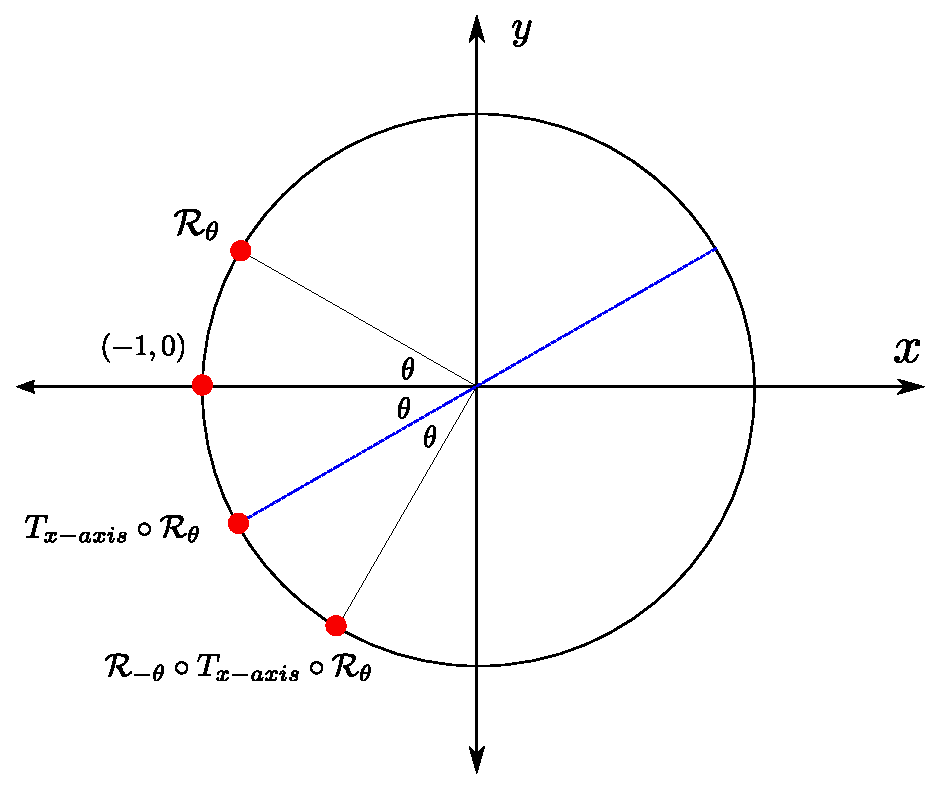
\includegraphics[scale=0.6]{chapters/images/13.7.eps}
\caption{}
\end{figure} 
\subsubsection*{Case 2 - Only rotations}
We will now show that there are no subgroups of $SO(3)$ which can be normal with respect to $O(3)$. We could do this using a similar technique to Case 1, but it is a little messy. A more elegant method is to use quaternions. \\ \\ We will need some facts which Penrose doesn't explicitly state, but could be derived if clever enough.
\begin{itemize}
\item The quaternion $\mathbb{V}=\cos \frac{\theta}{2}+\sin \frac{\theta}{2}(v_1\textbf{i}+v_{2}\textbf{j}+v_{3}\textbf{k})=\cos \frac{\theta}{2}+\sin \frac{\theta}{2}\mathbf{V}$ where $\mathbf{V}$ is a unit vector, represents a rotation of $\theta$ about the axis $\mathbf{V}$.
\item Suppose we have some 3-d vector $\mathbf{W}$. Then $\mathbf{W}'=\mathbb{V}\mathbf{W}\mathbb{V}^{-1}$ is $\mathbf{W}$ rotated about $\mathbf{V}$ by an angle $\theta$.
\end{itemize}
Now suppose there exists a non-trivial normal subgroup of $SO(3)$. Then it must contain some rotation represented by a quaternion of the form $\mathbb{W}=\cos \frac{\phi}{2}+\sin \frac{\phi}{2}(w_1\textbf{i}+w_{2}\textbf{j}+w_{3}\textbf{k})=\cos \frac{\phi}{2}+\sin \frac{\phi}{2}\mathbf{W}$. Obviously $\phi\neq 2\pi$, and let us assume also for now that $\phi\neq \pi$. Now for the subgroup containing $\mathbb{W}$ to be normal, it must also contain all elements of the form \begin{align*}
\mathbb{V}\mathbb{W}\mathbb{V}^{-1}=\mathbb{V}(\cos \frac{\phi}{2}+\sin \frac{\phi}{2}\mathbf{W})\mathbb{V}^{-1}=\cos \frac{\phi}{2}\cdot 1+\sin \frac{\phi}{2}\mathbb{V}\mathbf{W}\mathbb{V}^{-1}
\end{align*}
As $\mathbb{V}$ is arbitrary, $\mathbb{V}\mathbf{W}\mathbb{V}^{-1}$ is an arbitrary rotation of the unit vector $\mathbf{W}$, and so $\mathbb{V}\mathbf{W}\mathbb{V}^{-1}$ is also an arbitrary vector. Hence the subgroup containing the rotation $\mathbb{W}$ must also contain rotations of $\phi$ about \emph{every rotation axis}. \\ \\ Now we demand that this group be closed, and show that this further requirement generates the whole of $SO(3)$.  \\ \\ We know that our potential normal subgroup contains a rotation of $\phi$ about the $z-$axis. Now we need to show that for any $\theta$, a rotation of $\theta$ about the $z-$axis must also be in our subgroup. This is easy. Suppose we have a point $\mathbf{A}=(0,\frac{\pi}{2})$ and a point $\mathbf{B}=(\theta,\frac{\pi}{2})$.  


\subsection{13.9 $\bigstar \bigstar $}
Let us denote the order of the group $\mathcal{G}$ by $|\mathcal{G}|$. We are trying to show that $|\mathcal{G}/\mathcal{S}|=|\mathcal{G}|/|\mathcal{S}|$. Now let $H$ be the set $H=\mathcal{G}-\mathcal{S}$, ie. all the elements of $\mathcal{G}$ not in $\mathcal{S}$. We will need the following simple results:
\begin{itemize}
\item[1.] If $s\in\mathcal{S}$, then $s*\mathcal{S}=\mathcal{S}$, the identity element.
\item[2.] The order of $H$ is $|H|=|\mathcal{G}|-|\mathcal{S}|$.
\item Suppose $h_1\in H$ and $s\in\mathcal{S}$. Then $h_1* s\in H$. This is easy to show, as suppose that $h_1*s\in \mathcal{S}$. Then $h_1 *s*s^{-1}=h_1\in \mathcal{S}$, which is a contradiction.
\item[3.] Let $h_1\in H$. Then $h_1$ maps each element of $\mathcal{S}$ into a unique element of $H$. Uniqueness is easy to show, as $h_1*s_1=h_1*s_2\implies s_1=s_2$
\item[4.] Let $H_1=h_1*\mathcal{S}$. Then $|H_1|=|\mathcal{S}|$. This follows from the last two points.
\item[5.] Let $H_1=h_1*\mathcal{S}$. Now suppose $h_2\notin H_1$. Then $h_2*s \notin H_1$. To see this, suppose there is some $s_1,s_2\in \mathcal{S}$, such that $h_1*s_1=h_2*s_2$. Then $h_2=h_1*s_1*s^{-1}_{2}$. But there is some $s\in \mathcal{S}$ such that $s=s_1*s^{-1}_{2}$. Then $h_2=h_1*s\in H_1$. Contradiction!
\end{itemize}
We can thus conclude that after applying each of the elements of $H$ to $\mathcal{S}$, we get a collection of sets $H_1,H_2,\ldots H_n$. These sets are non-intersecting (from point 5.) and each of order $|\mathcal{S}|$ (point 4.). Thus the number $n$ of of these sets must be 
$$n=\frac{|H|}{|\mathcal{S}|}=\frac{|\mathcal{G}|-|\mathcal{S}|}{|\mathcal{S}|}=\frac{|\mathcal{G}|}{|\mathcal{S}|}-1$$
Each of these sets is an element of $\mathcal{G}/\mathcal{S}$ But we haven't counted in $\mathcal{S}$, which is the identity element. Including this, we get
$$|\mathcal{G}/\mathcal{S}|=\frac{|\mathcal{G}|}{|\mathcal{S}|}-1+1=\frac{|\mathcal{G}|}{|\mathcal{S}|}$$
From another perspective, we have shown that the sets $g*\mathcal{S}$, where $g\in \mathcal{G}$, form a partition of $\mathcal{G}$, meaning that either $(g_1*\mathcal{S})\cap (g_2*\mathcal{S})=\emptyset$ or $(g_1*\mathcal{S})= (g_2*\mathcal{S})$, and that the union of all these sets is just the set $\mathcal{G}$. Knowing this, and that each set $g\in \mathcal{G}$ has order $\mathcal{S}$, the result follows easily.   \\ \\ \textbf{Note:} Sharp-eyed readers might wonder what would happen if $|\mathcal{S}|$ does not divide $|\mathcal{G}|$. Surely a group can't have a fractional order! Indeed not. The resolution to the problem is that the order of any subgroup of a group $\mathcal{G}$, must divide the order of the group $\mathcal{G}$. This is known as \emph{Lagrange's Theorem}, which we have effectively proven. A simple consequence, for example, is that a group of prime order cannot have any (non-trivial) subgroups. pp


\subsection{13.17 $\bigstar \bigstar $}
Suppose there exists $\mathbf{v}_1\neq \mathbf{0}$ such that $\mathbf{T}\mathbf{v}_1=\mathbf{0}$. Now suppose our vector space $\mathbb{V}$ is of dimension $n$. Then we can always find a set of $n$ linearly independent vectors $\{\mathbf{v}_1,\mathbf{v}_2,\ldots,\mathbf{v}_n\}$ such that an arbitrary vector $\mathbf{w}\in\mathbb{V}$ can be written as a linear combination of these vectors.\\ Now let $\mathbb{W}_{\mathbf{T}}=\{\mathbf{T}\mathbf{u}:\mathbf{u}\in \mathbb{V}\}$. An arbitrary element of $\mathbb{W}_{\mathbf{T}}$ can be written
\begin{align*}
\mathbf{T}\mathbf{w}&=\mathbf{T}(\alpha_1 \mathbf{v}_1+\alpha_2 \mathbf{v}_2+\ldots \alpha_n \mathbf{v}_n)\\
&=\alpha_1 \mathbf{T}\mathbf{v}_1+\alpha_2 \mathbf{T}\mathbf{v}_2+\ldots \alpha_n \mathbf{T}\mathbf{v}_n\\
&=\mathbf{0}+\alpha_2 \mathbf{T}\mathbf{v}_2+\ldots \alpha_n \mathbf{T}\mathbf{v}_n\\
\end{align*} 
And so the set $\{\mathbf{T}\mathbf{v}_2,\mathbf{T}\mathbf{v}_3,\ldots  ,\mathbf{T}\mathbf{v}_n\}$ forms a basis for $\mathbb{W}_{\mathbf{T}}$. But it has only $n-1$ elements, and so its dimension is smaller than that of $\mathbb{V}$, and hence is singular.\\ \\ I think Penrose made a mistake with his hint, as he no where mentions the determinant condition, which is that $\mathbf{T}$ is singular iff $\det \mathbf{T}=0$. Then a simple fact about determinants is that iff you swop two rows or columns, then the determinant picks up a minus sign. But if there are two rows which are the same, then swopping them leaves $\mathbf{T}$ unchanged, and so $\det \mathbf{T}=-\det\mathbf{T}\implies \det \mathbf{T}=0$. It is also obvious that if there is a row or column of zeroes, then the determinant is also zero.


\subsection{13.18 $\bigstar \bigstar $}
I am not completely sure what Penrose means by `not using explicit expressions'. \\ \\ The key fact we will use is that any bijective map has an inverse. (This should be intuitively obvious.) We assume that $\mathbf{T}$ is non-singular. In our case, we obviously don't have to worry about $\mathbf{T}$ being surjective (onto). So let us show it is injective (one-to-one). Now suppose $\mathbf{T}\mathbf{v}=\mathbf{T}\mathbf{u}\implies \mathbf{T}(\mathbf{v}-\mathbf{u})=\mathbf{0}
$. But $\mathbf{T}$ is non-singular, and so $\mathbf{v}-\mathbf{u}=\mathbf{0}\implies \mathbf{v}=\mathbf{u}$ and so $\mathbf{T}$ is injective, and hence bijective, and hence has an inverse.\\ \\ Another way of seeing this is to note that two vector spaces $\mathbb{V}$ and $\mathbb{W}$ of the same dimension are basically the same, as they have an equivalent number of basis vectors. One can easily find a linear map mapping the basis vectors of $\mathbb{W}$ to basis vectors of $\mathbb{V}$. Then the inverse of this map simply maps the basis vectors of $\mathbb{V}$ to those of $\mathbb{W}$.


\subsection{13.25 $\bigstar\bigstar\bigstar$}
We present three proofs here. The first is what I think Penrose wanted, and relies on the Jordan Canonical form, which is reffered to in Footnote \textbf{12} (whilst the second and third do not). The second is what I consider the most elegant, whilst the third I found somewhere and relies on the least amount of matrix algebra facts.\\ \\ For the first and second proof, we need the fact that for any $n\times n$ matrix $\mathbf{A}$, which has eigenvalues $\lambda_1,\lambda_2,\ldots,\lambda_n$, 
\begin{align*}
\det \mathbf{A}&=\lambda_1\lambda_2\ldots\lambda_n\\
\text{trace}\mathbf{A}&=\lambda_1+\lambda_2+\ldots+\lambda_n
\end{align*} 
which we found in Question \textbf{[13.27]}.
\subsubsection*{Proof 1}
Following Penrose, we first assume the eigenvalues of \textbf{A}, $\lambda_1,\lambda_2,\ldots,\lambda_n$ are distinct, and show that 
$$\det e^\textbf{A}=e^{\text{trace}\,\textbf{A}}$$ 
holds for this case. We immediately have, iff \textbf{A} is an $n\times n$ matrix, that
$$e^{\text{trace}\,\textbf{A}}=e^{\lambda_1+\lambda_2+\ldots+\lambda_n}$$
As the eigenvalues are distinct, we can always choose the eigenvectors of \textbf{A} as the basis, and so express \textbf{A} in the Canonical form. In this basis, it can easily be seen that
$$\textbf{A}^k=
\begin{pmatrix} 
\lambda_{1}^{k}&0 &\ldots&0\\
0&\lambda_{2}^{k}&\ldots&0\\
\vdots & \vdots & \ldots &\vdots \\
0&0&\ldots &\lambda_{n}^{k}
\end{pmatrix}$$
Hence
\begin{align*}
\det e^\textbf{A}&=\det \left ( 1+\textbf{A}+\frac{\textbf{A}^2}{2!}+\ldots\right)\\
&=\det \begin{pmatrix} 
1+\lambda_{1}+\frac{\lambda_{1}^{2}}{2!}+\ldots&0 &\ldots&0\\
0&1+\lambda_{2}+\frac{\lambda_{2}^{2}}{2!}+\ldots&\ldots&0\\
\vdots & \vdots & \ldots &\vdots \\
0&0&\ldots &1+\lambda_{n}+\frac{\lambda_{n}^{2}}{2!}+\ldots
\end{pmatrix}\\
&=\det \begin{pmatrix} 
e^\lambda_1&0 &\ldots&0\\
0&e^\lambda_2&\ldots&0\\
\vdots & \vdots & \ldots &\vdots \\
0&0&\ldots &e^\lambda_n
\end{pmatrix}\\
&=e^{\lambda_1+\lambda_2+\ldots+\lambda_n}=e^{\text{trace}\,\textbf{A}}
\end{align*}
Now when the eigenvalues are degenerate, the we cannot necessarily express \textbf{A} in the Canonical form. But according to Footnote \textbf{12}, we can find a basis for \textbf{A} such that it will be in the Canonical form with at most some ones in the next diagonal.\\ This Jordan Canonical form is evidently an upper triangular matrix. Two easy to see facts about upper triangular matrices are that iff \textbf{A} is upper triangular, then $\det (\textbf{A})=a_{11}a_{22}\ldots a_{nn}$, and the product of two upper triangular matrices is also upper triangular. The last thing we note is that iff \textbf{A} and \textbf{B} are upper triangular, and \textbf{A}\textbf{B}=\textbf{C}, then $c_{ii}=a_i\, b_i$. Using these facts, it is easy to see that the proof for Canonical matrices will extend exactly to matrices in the Jordan canonical form, and so degeneracies in the eigenvalues can't falsify the expression $\det e^\textbf{A}=e^{\text{trace}\,\textbf{A}}$.\\ \\ 

\subsubsection*{Proof 2}
The method of this proof is to find the eigenvalues of $e^{\mathbf{A}}$, and then find $\text{det}\,e^\mathbf{A}$. Now suppose \textbf{A} is again an $n\times n$ matrix with eigenvalues $\lambda=\lambda_1,\lambda_2,\ldots,\lambda_n$. Also, \textbf{v} is an $n\times 1$ column vector. Then we immediately have that $\mathbf{A}^n\mathbf{v}=\lambda^n\mathbf{v}$, and so
\begin{align*}
e^\mathbf{A}\mathbf{v}&=\left (\mathbf{I}+\frac{\mathbf{A}}{1!}+\frac{\mathbf{A}^2}{2!}+\frac{\mathbf{A}^3}{3!}+\ldots\right )\mathbf{v}\\
&=\left (\mathbf{I}\mathbf{v}+\frac{\mathbf{A}\mathbf{v}}{1!}+\frac{\mathbf{A}^2\mathbf{v}}{2!}+\frac{\mathbf{A}^3\mathbf{v}}{3!}+\ldots\right )\\
&=\left (1\cdot\mathbf{v}+\frac{\lambda\cdot\mathbf{v}}{1!}+\frac{\lambda^2\cdot\mathbf{v}}{2!}+\frac{\lambda^3\cdot\mathbf{v}}{3!}+\ldots\right )\\
&=e^\lambda \cdot \mathbf{v}\\
\end{align*}
So iff $\lambda$ is an eigenvalue of \textbf{A}, then $e^\lambda$ is an eigenvalue of $e^\mathbf{A}$. Hence 
\begin{align*}
\text{det}\,e^\mathbf{A}&=e^{\lambda_1}\cdot e^{\lambda_2}\cdot \ldots \cdot e^{\lambda_n}\\
&=e^{\lambda_1+\lambda_2+\ldots +\lambda_n}\\
&=e^{\text{trace}\mathbf{A}}
\end{align*}


\subsubsection*{Proof 3}
Another interesting proof is one I found in t'Hoofts Lie Algebra notes. We know that for a real number $x$, $$e^x=\lim_{m\to \infty} \left (1+\frac{x}{m}\right)^m$$
Now the same holds iff we replace the $x$ with a matrix \textbf{A} and the 1 with the identity matrix \textbf{I}. This is because we prove the identity in the real case using the binomial theorem, and as the only elements in the binomial expansion for the matrix case are \textbf{A} and \textbf{I}, which commute with themselves and each other, and so they behave just like real numbers. So the real proof will hold for the matrix case too. Now let $m$ be a natural number. Then using $\det (\textbf{A}\textbf{B})=\det (\textbf{A})\det(\textbf{B})$,
\begin{align*}
\det e^\textbf{A}&= \lim_{m\to \infty}\left[ \det \left (\textbf{I}+\frac{\textbf{A}}{m}\right)^m\right]=\lim_{m\to \infty}\left[ \det \left (\textbf{I}+\frac{\textbf{A}}{m}\right)\right]^m
\end{align*}
Now we are only interested in terms of order $1/m$, nothing $\mathcal{O}(1/m^2)$. Now 
\begin{align*}
\det \left (\textbf{I}+\frac{\textbf{A}}{m}\right)&=(1+\frac{a_{11}}{m})(1+\frac{a_{22}}{m})\ldots (1+\frac{a_{nn}}{m})+\mathcal{O}(\frac{1}{m^2})\\
&=1+\frac{1}{m}\left(a_{11}+a_{22}+\ldots+a_{nn}\right)+\mathcal{O}(1/m^2)\\
&=1+\frac{1}{m}\text{trace}(\textbf{A})+\mathcal{O}(1/m^2)
\end{align*}
as the off diagonal elements in the determinant are obviously all of order $\mathcal{O}(1/m^2)$. Then we finally have 
\begin{align*}
\det e^\textbf{A}=\lim_{m\to \infty}\left[ \det \left (\textbf{I}+\frac{\textbf{A}}{m}\right)\right]^m&=\lim_{m\to \infty}\left[ 1+\frac{1}{m}\text{trace}(\textbf{A})+\mathcal{O}(1/m^2)\right]^m\\
&=e^{\text{trace}\mathbf{A}}
\end{align*}
as in the limit $m\to \infty$ the terms $\mathcal{O}(1/m^2)$ do not contribute in the above.


\subsection{13.27 $\bigstar$}
The proof of these identities is trivial iff one notes two facts: The determinant and trace of matrices are basis-independant quantities, and that one can always choose a basis so that the matrix is in the \emph{Jordaan Normal form}, which Penrose alludes to in his Notes 13.12. \\ \\
I am not sure whether Penrose wanted us to use this Jordaan normal form, or rather just prove it for matrices expressible in the Canonical form on pg. 265, or there is some other way involving neither of these.





\subsection{13.28 $\bigstar\bigstar\bigstar$}
To do the proof, we need some definitions. What is meant by an $n$-dimensional vector space? Motivated by the vague definition of Chapter 11.1 pg. 199, we say a vector space $\mathbf{V}$ is of dimension $n$ iff there are $n$ linearly independent vectors $\mathbf{k}_1,\mathbf{k}_2,\ldots \mathbf{k}_n$ of $\mathbf{V}$, which span\footnote{A set of vectors $\mathbf{k}_1,\mathbf{k}_2,\ldots \mathbf{k}_n$ \emph{span} the space $\mathbf{V}$ iff every element of $\mathbf{V}$ is equal to a linear combination of the vectors $\mathbf{k}_1,\mathbf{k}_2,\ldots \mathbf{k}_n$} $\mathbf{V}$. \\ \\ Now suppose we have a vector $\mathbf{v}\in \mathbf{V}$, where $\mathbf{k}$ is an $n$-dimensional vector space. Then from our definition, there exists some vectors $\mathbf{k}_1,\mathbf{k}_2,\ldots \mathbf{k}_n$ such that
$$\mathbf{v}=b_1\mathbf{k}_1+b_2\mathbf{k}_2+\ldots +b_n\mathbf{k}_n$$    
Now what we need to prove, is that given any other set of $n$ linearly independant vectors $\mathbf{e}_1,\mathbf{e}_2,\ldots \mathbf{e}_n$, there exist some set of constants $x_1,x_2,\ldots,x_n$ such that
$$\mathbf{v}=x_1\mathbf{e}_1+x_2\mathbf{e}_2+\ldots +x_n\mathbf{e}_n$$ 
Now we note that as the set $\mathbf{k}_1,\mathbf{k}_2,\ldots \mathbf{k}_n$ spans $\mathbf{V}$, we can write $\mathbf{e}_i=\sum^{n}_{j=1}a_{ij} \mathbf{k}_j$. And so 
\begin{align*}
\mathbf{x}=x_1\mathbf{e}_1+x_2\mathbf{e}_2+\ldots +x_n\mathbf{e}_n&=\sum_{i=1}^{n} x_i\left(\sum^{n}_{j=1}a_{ij} \mathbf{k}_j\right)\\
&=\mathbf{k}_1\left(\sum_{i=1}^{n}x_i a_{i1}\right)+\mathbf{k}_2\left(\sum_{i=1}^{n}x_i a_{i2}\right)+\ldots+\ \mathbf{k}_n\left(\sum_{i=1}^{n}x_i a_{in}\right)
\end{align*}
as we can interchange the order of multiple sums. We can write this much more elegantly if represent $\mathbf{x}$ with the column matrix $\mathbf{x}=(x_1\ x_2 \ \ldots\ x_n)^T$ in the basis $\mathbf{e}_1,\mathbf{e}_2,\ldots \mathbf{e}_n$, and also $\mathbf{x}'=\mathbf{x}=(x_1\ x_2 \ \ldots\ x_n)^T$ in the basis $\mathbf{k}_1,\mathbf{k}_2,\ldots \mathbf{k}_n$. Then
$$\mathbf{x}=\mathbf{A} \mathbf{x}'$$
where
$$\mathbf{A}=\begin{pmatrix} a_{11} & a_{12} &\ldots & a_{1n}\\
a_{21} & a_{22} &\ldots & a_{2n}\\
\vdots & \vdots & &\ldots \\
a_{n1}&a_{n2}&\ldots &a_{nn}\end{pmatrix}$$
We have simply proven here what Penrose states at the top of page 265, the transformation sending a vector from one base to another is linear.\\ Now we want to show that we can pick $x_1,x_2,\ldots,x_n$ such that $\mathbf{v}=\mathbf{x}$. To do this, we need to satisfy
$$\mathbf{v}=\mathbf{x}=\mathbf{A} \mathbf{x}'$$
We can certainly do this iff $\mathbf{A}$ has an inverse, as then $$\mathbf{x}'=\mathbf{A}^{-1} \mathbf{v}$$
A necessary and sufficient condition for the inverse to exist is that iff for some vector \textbf{z},  $\mathbf{A}\mathbf{z}=\mathbf{0}$ then $\mathbf{z}=\mathbf{0}$, and nothing else. It is obvious why this is a necessary condition, as we always have, for a linear transformation $\mathbf{A}$ that $\mathbf{A}\mathbf{z}=0$ when $\mathbf{z}=\mathbf{0}$. But if there is another $\mathbf{z}\neq\mathbf{0}$ such that $\mathbf{A}\mathbf{z}=0$, then $\mathbf{A}$ is not a one-to-one function, and there can't be an inverse.\footnote{We can prove the sufficient part as follows: $\mathbf{A}^{-1}$ exists iff $\mathbf{A}$ is non-singular. We then use a theorem which says that a matrix $\mathbf{A}$ is non-singular iff its nullspace only contains the zero vector.} \\ \\ Using the above fact, we see that 
$\mathbf{x}=\mathbf{A} \mathbf{x}'=0$ implies that $\mathbf{x}=(0,0,\ldots,0)^T$ due to linear independence, and then $\mathbf{x}'=(0,0,\ldots,0)^T$. So there is only one solution to $\mathbf{A} \mathbf{x}'=0$, namely the zero vector, and so $\mathbf{A}$ has an inverse.\\ And so we have shown what was needed, that for any $\mathbf{v}\in\mathbf{V}$, we can write $\mathbf{v}=x_1\mathbf{e}_1+x_2\mathbf{e}_2+\ldots +x_n\mathbf{e}_n$ for where $\mathbf{e}_1,\mathbf{e}_2,\ldots \mathbf{e}_n$ are an arbitrary linearly independen set of vectors.  \\ \\ Finally, we need to show uniqueness. Suppose we have
\begin{align*}
\mathbf{x}=x_1\mathbf{e}_1+x_2\mathbf{e}_2+\ldots +x_n\mathbf{e}_n&=y_1\mathbf{e}_1+y_2\mathbf{e}_2+\ldots +y_n\mathbf{e}_n\\
\implies\ \ \ \   (x_1-y_1)\mathbf{e}_1+(x_2-y_2)\mathbf{e}_2+\ldots +(x_n-y_n)\mathbf{e}_n&=0
\end{align*}
but the vectors are linearly independent, and so $(x_i-y_i)=0\implies x_i=y_i$, and so $\mathbf{x}$ is uniquely represented in any particular linearly independent basis.










\newpage
\section{16. The ladder of infinity}
% --------------------------------------
% Chapter 16 Solutions
% --------------------------------------


\subsection{16.16 $\bigstar \bigstar\bigstar $}
We need to prove both ways of the implication.
\subsection*{1. Recursive $\implies$ recursively enumerable}
We suppose that the set $S$ is recursive. Then there exists a Turing machine $\mathbf{T}_S(n)$ such that $\mathbf{T}_S(n)=1$ iff $n\in S$ and $\mathbf{T}_S(n)=0$ iff $n\notin S$. Now define another Turing machine $\mathbf{U}_S(n)$ with
\begin{itemize}
\item[] $\mathbf{U}_S(n)=n$ iff $\mathbf{T}_S(n)=1$ \\ $\mathbf{U}_S(n)$ does not halt when $\mathbf{T}_S(n)=0$
\end{itemize} 
Now it is evident that $\mathbf{U}_S(\mathbb{N})=S$, as for those $n$ for which $\mathbf{U}_S(n)$ doesn't halt, no output is produced by the machine, and so has no effect on the set of all outputs of $\mathbf{U}_S(n)$, in our case $S$. Hence our set $S$ is produced by the action of a Turing machine ($\mathbf{U}_S(n)$) and hence is recursively enumerable.\\ \\ It is now trivial to see that the set $\overline{S}=\mathbb{N}-S$ is also recursively enumerable, as we just modify $\mathbf{U}_S(n)$ so that $\mathbf{U}_S(n)=n$ iff $\mathbf{T}_S(n)=0$ and $\mathbf{U}_S(n)$ does not halt when $\mathbf{T}_S(n)=1$.

\subsection*{2. recursively enumerable $\implies$ recursive  }
We suppose that $S$ and $\overline{S}$ are recursively enumerable. Thus there exist Turing machines $\mathbf{T}_S$ and  $\overline{\mathbf{T}}_S$ such that $\mathbf{T}_S(\mathbb{N})=S$ and $\overline{\mathbf{T}}_S(\mathbb{N})=\overline{S}$. Now for $S$ to be recursive, we must be able to construct another Turing machine $\mathbf{V}_S(n)$ which can test tell whether or not $n\in S$. To do this, $\mathbf{V}_S(n)$ runs $\mathbf{T}_S(0)=a$ and  $\overline{\mathbf{T}}_S(0)=b$. If $a=n$, then $\mathbf{V}_S(n)=1$, and iff $b=n$, then $\mathbf{V}_S(n)=0$. If neither $a$ nor $b$ equal $n$, then it tries $\mathbf{T}_S(1)=a$ and  $\overline{\mathbf{T}}_S(1)=b$ and repeats the previous steps. If it still hasn't halted, it tries  $\mathbf{T}_S(2)$ and  $\overline{\mathbf{T}}_S(2)$, etc. Eventually it will halt, and spit out either 1 or 0. Hence $S$ is recursive. \\ \\ We can see why both $S$ and $\overline{S}$ must be recursively enumerable for $S$ to be recursive. If only $S$ were recursively enumerable, and not $\overline{S}$, then we could only check whether $n\in S$. If indeed $n\in S$, then our search will end. But if $n\notin S$, then we could never establish this, as our search would carry on forever.    


\newpage
\section{19. The Classical Fields of Maxwell and Einstein}
% --------------------------------------
% Chapter 19 Solutions
% --------------------------------------


\subsection{19.5 $\bigstar \bigstar$}
Below is a diagrammatic proof that $*(*\mathbf{F})=-\mathbf{F}$. An explanation:
\begin{itemize}
\item[e)] Swopping two indices in the levi-civita tensor picks up a minus sign.
\item[g)] Two indices are swopped, picking up two minus signs.
\item[h)] Using one of the identities in Penroses Fig 12.18.
\item[i)] Using the fact that $\mathbf{F}$ is an antisymmetric tensor.
\end{itemize}
Using this, we have that
\begin{align*}
*(^\pm \mathbf{F})&=\frac{1}{2}*(\mathbf{F}\mp i*\mathbf{F})\\
&=\frac{1}{2}(*\mathbf{F}\mp i**\mathbf{F})\\
&=\frac{1}{2}(*\mathbf{F}\pm i\mathbf{F})\\
&=\frac{i}{2}((-i)*\mathbf{F}\pm \mathbf{F})\\
&=\pm i^\pm \mathbf{F}
\end{align*}
\begin{figure}\label{e}
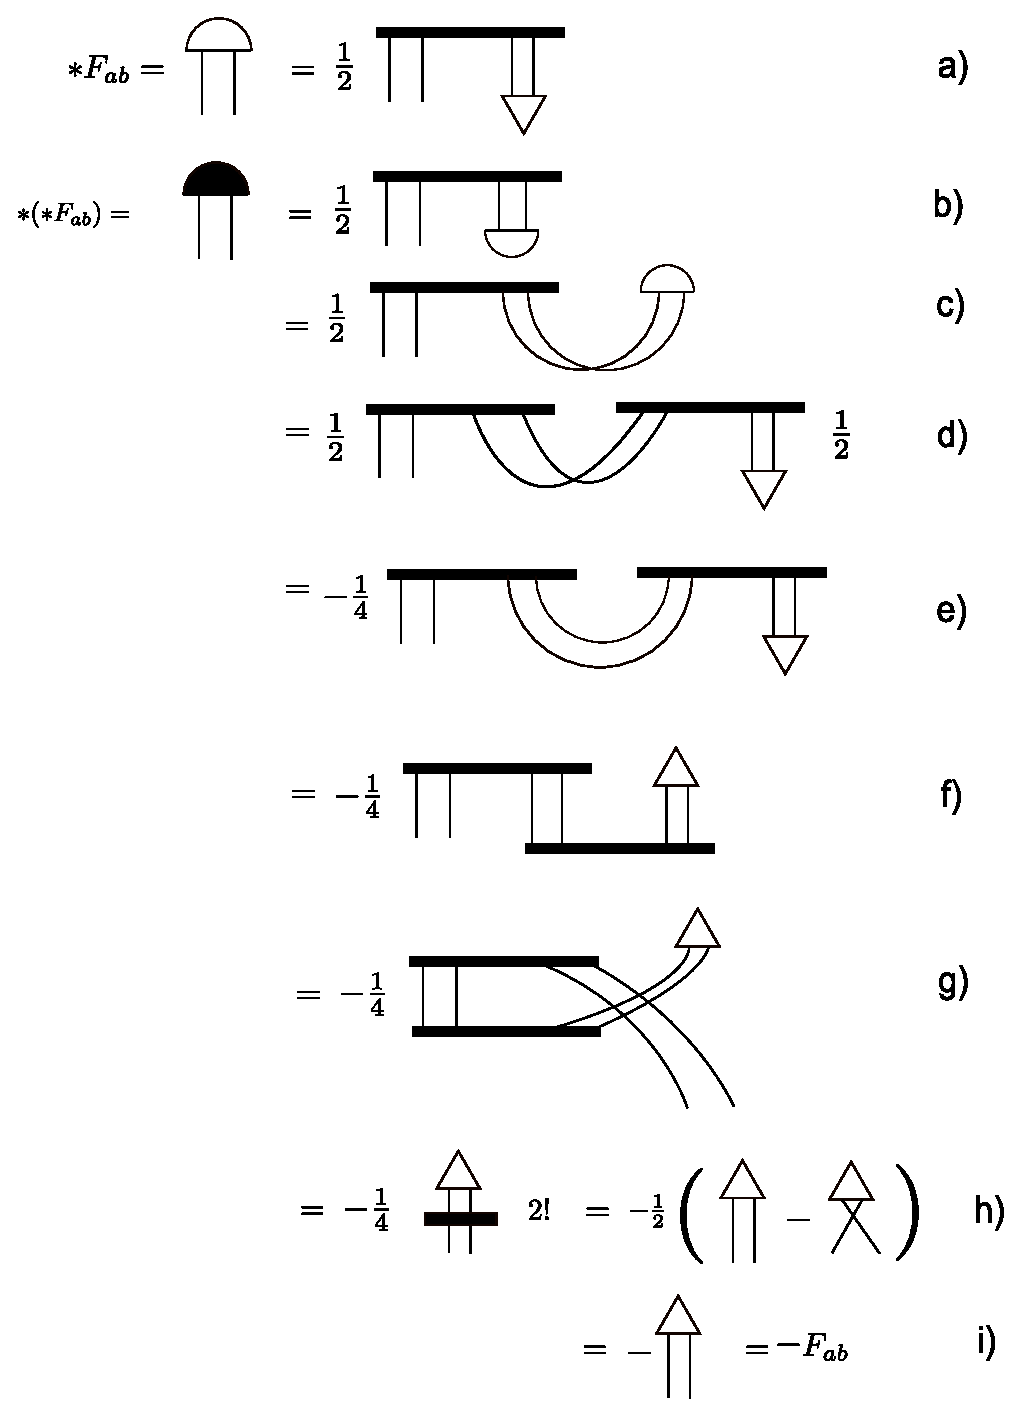
\includegraphics[scale=0.7]{chapters/images/19.5.eps}
\caption{Diagrammatic proof of $*(*\mathbf{F})=-\mathbf{F}$ }
\end{figure} 


\newpage
\section{20. Lagrangians and Hamiltonians}
% --------------------------------------
% Chapter 20 Solutions
% --------------------------------------


\subsection{20.9 $\bigstar\bigstar\bigstar$}
We need to show that iff the $n\times n$ matrices $\mathbf{P}$ and $\mathbf{Q}$ are positive-definite, then the product  $\mathbf{W}=\mathbf{P}\mathbf{Q}$ must have positive eigenvalues. So suppose the vector $\mathbf{v}$ is an eigenvector of $\mathbf{W}$ with eigenvalue $\lambda$. Then 
\begin{align*}
(\mathbf{P}\mathbf{Q})\mathbf{v}&=\lambda\mathbf{v}\\
\implies \ \  \ \ \mathbf{Q}\mathbf{v}&=\lambda \mathbf{P}^{-1}\mathbf{v}\\
\implies \mathbf{v}^T\mathbf{Q}\,\mathbf{v}&=\lambda \mathbf{v}^T\mathbf{P}^{-1}\mathbf{v}\\
\implies \qquad  \lambda&= \frac{\mathbf{v}^T\mathbf{Q}\,\mathbf{v}}{\mathbf{v}^T\mathbf{P}^{-1}\mathbf{v}}>0
\end{align*}
As $\mathbf{Q}$ is positive-definite, we immediately have that $\mathbf{v}^T\mathbf{Q}\,\mathbf{v}>0$. Now there are two things we need to prove for us to be able to conclude in the above that $\lambda>0$:
\begin{itemize}
\item $\mathbf{v}^T\mathbf{P}^{-1}\,\mathbf{v}>0$, ie. that the inverse of a positive-definite matrix is also positive-definite. 
\item Any positive-definite matrix actually has an inverse.
\end{itemize}  
The way to see the first part is by changing our basis, $\mathbf{v}= \mathbf{P}^{-1}\,\mathbf{x}$. We note that $\mathbf{P}$ is a symmetric matrix, which means that its inverse is also symmetric.\footnote{This is easy to see. $(\mathbf{P}\mathbf{P}^{-1})^T=(\mathbf{P}^{-1})^T\mathbf{P}^T=(\mathbf{P}^{-1})^T\mathbf{P}=\mathbf{I}$. As inverses are unique, $(\mathbf{P}^{-1})^T=\mathbf{P}^{-1}$ and hence $\mathbf{P}^{-1}$ is symmetric. } Hence 
$$0<\mathbf{v}^T\mathbf{P}\,\mathbf{v}= \mathbf{x}^T(\mathbf{P}^{-1})^T\mathbf{P}\mathbf{P}^{-1}\,\mathbf{x}=\mathbf{x}^T(\mathbf{P}^{-1})^T\,\mathbf{x}=\mathbf{x}^T\mathbf{P}^{-1}\,\mathbf{x}$$ As $\mathbf{x}$ is an arbitrary non-zero vector, we have that $\mathbf{P}^{-1}$ is positive-definite.\\ \\ The second part is quite simple. It is easy to see\footnote{If you can't immediately see this, then this can be shown as follows. Let $\mathbf{P}$ positive-definite, with eigenvector $\mathbf{v}$ and eigenvalue $\lambda$. Then $$\mathbf{v}^T\mathbf{P}\mathbf{v}=k>0\implies\mathbf{v}^T\mathbf{v}\lambda =k\implies \lambda=\frac{k}{\mathbf{v}^T\mathbf{v}}>0$$ as obviously $\mathbf{v}^T\mathbf{v}>0$ } that any eigenvalue $\lambda_i$ of a positive-definite matrix $\mathbf{P}$ satisfies $\lambda_i>0$. But $\det \mathbf{P}=\lambda_1\lambda_2\ldots\lambda_n>0\neq 0$, and hence $\mathbf{P}$ is non-singular and has an inverse.


\subsection{20.12 $\bigstar\bigstar\bigstar$}
There is in fact an easy proof. It is obvious that $\mathbf{r}^T\mathbf{Q}\,\mathbf{q}= k$. We need to show that $k=0$. \\ \\ Assume $\mathbf{W}\mathbf{r}=\phi^2\mathbf{r}$ and $\mathbf{W}\mathbf{v}=\omega^2\mathbf{v}$, where $\mathbf{W}=\mathbf{P}\mathbf{Q}$, and $\omega\neq \phi$. Then 
\begin{align*}
\mathbf{r}^T\mathbf{Q}\,\mathbf{q}=k&\implies  (\phi^2\mathbf{r})^T\mathbf{Q}\,(\omega^2\mathbf{q})=k\phi^2\omega^2\\
&\implies (\mathbf{W}\mathbf{r})^T\mathbf{Q}\,(\mathbf{W}\mathbf{q})=k\phi^2\omega^2\\
&\implies (\mathbf{r}^T\mathbf{Q}^T\mathbf{P}^T) \mathbf{Q}\,(\mathbf{P}\mathbf{Q}\,\mathbf{q})=k\phi^2\omega^2\\
&\implies \mathbf{r}^T(\mathbf{Q}\mathbf{P} \mathbf{Q}\,\mathbf{P}\mathbf{Q})\,\mathbf{q}=k\phi^2\omega^2\\
&\implies \mathbf{r}^T\mathbf{Q}(\mathbf{W}\mathbf{W}\mathbf{q})=k\phi^2\omega^2\\
&\implies \mathbf{r}^T\mathbf{Q}(\omega^4\mathbf{q})=k\phi^2\omega^2\\
&\implies \mathbf{r}^T\mathbf{Q}\mathbf{q}=\frac{k\phi^2}{\omega^2}\\
&\implies \frac{k\phi^2}{\omega^2}=k
\end{align*}
But this is only satisfied if $\omega=\phi$ or if $k=0$.\footnote{What about if either $\omega$ or $\phi$ are zero? We have that $\omega,\phi\neq 0$, as we showed that the  eigenvalues of $\mathbf{W}$ can't equal zero in question 20.9.}  As one of the assumptions was that $\omega\neq\phi$, we must have that $k=0$ and hence $\mathbf{r}^T\mathbf{Q}\,\mathbf{q}= 0$, as we wanted to show.


\newpage
\section{21. The Quantum Particle}
% --------------------------------------
% Chapter 21 Solutions
% --------------------------------------


\subsection{21.1 $\bigstar$}
\begin{align*}
(1+D^2)\cos x&=\cos x+D^2\cos x\\
&=\cos x- D \sin x\\
&=\cos x-\cos x \\
&=0
\end{align*}
The other one is done exactly like this one.


\subsection{21.2 $\bigstar\bigstar$}
The first fact we will need is that $y(x)=A\cos x + B\sin x$ is the most general solution\footnote{I am not sure how to show this in an elementary way. The standard approach is to show that $\cos x$ and $\sin x$ are linearly independant, and so span the solution space of the second-order differential equation, and hence their linear combination is the most general solution.} to 
$$(1+D^2)y(x)=0$$
Now suppose $y_1(x)$ and $y_p(x)$ are both solutions to $(1+D^2)y(x)=x^5$. Then
\begin{align*}
&(1+D^2)y_1=x^5=(1+D^2)y_p\\
\implies \ \ \ \ & (1+D^2)y_1-(1+D^2)y_p=0\\
\implies \ \ \ \ & (1+D^2)[y_1-y_p]=0\\
\implies \ \ \ \ & y_1-y_p=A\cos x + B\sin x
\end{align*}
Now suppose $y_1$ is the most general solution to $(1+D^2)y(x)=x^5$, and $y_p=x^5-20x^3+120x$. Then we have from the above that 
\begin{align*}
y_1&=A\cos x + B\sin x+y_p\\
&=(A\cos x + B\sin x)+(x^5-20x^3+120x)\end{align*}


\subsection{21.3 $\bigstar\bigstar\bigstar$}
Following Penrose, 
\begin{align*}
\frac{1}{1+D^2}(1+D^2)\cos x=\frac{1}{1+D^2}\cdot 0=0
\end{align*}
Thus applying the inverse operator does not give us $\cos x$, as we would want from a real inverse. \\ \\ Let $\mathcal{L}=a_0+a_1 D+a_2D^2+\ldots + a_nD^n$. We can see that in general, we cannot find an `inverse' for any differential equation of the form
$$\mathcal{L}y(x)=0$$
as the method always gives $y(x)=0$, which is obviously not the only solution. One of the reasons that the linear operator $\mathcal{L}$ does not have an inverse, is that it is not in general bijective. For example,
$$ (1+D^2)\cos x=0=(1+D^2)\sin x$$
Using the idea from the previous question, suppose $y_1$ and $y_p$ are solutions to the general differential equation $\mathcal{L} y(x) = f(x)$, then 
\begin{align*}
&\mathcal{L}y_1=f(x)=\mathcal{L}y_p\\
\implies \ \ \ \ & \mathcal{L}(y_1-y_p)=0\\
\end{align*}
Let $k(x)=y_1-y_p$. Then supposing $y_1$ to be the most general solution to $\mathcal{L} y(x) = f(x)$ and $y_p$ some other solution, we see that $y_1=k+y_p$.\\ \\ Now the key is to note is that our procedure of inverting $\mathcal{L}$ will always find a solution $y_p(x)$, but won't find $k(x)$. So the general procedure for solving equations of the form $\mathcal{L} y(x) = f(x)$ is to find an inverse $\mathcal{L}^{-1}$ using the series method in order to find $y_p\,$, and then solve the equation $\mathcal{L} k(x) = 0$ to obtain $k$, and hence obtain the general solution $y_1=y_p+k$.\\ \\
As for solving $\mathcal{L} k(x)=0$, this can be done in a variety of ways. One is by assuming $k$ is analytic, and so is of the form $k(x)=a_0+a_1x+a_2x^2+\ldots$, and then acting on the series with $\mathcal{L}$. With skill, one can find recursion relations, which allow one to find the form of the series $k(x)$.


\subsection{21.5 $\bigstar \bigstar$}
The normal procedure for constructing the most general solution this sort of partial differential equation is use the method of seperation of variables. Doing this would require a knowledge of Airy functions, which is hardly what Penrose must have in mind.\\ \\ Thus we look for a solution by intelligent guesswork. We think it may be some exponential depending on both $z$ and $t$. After playing around, you should find that
$$\Psi(t,z)=Ae^{-i(\frac{mg^2}{6\hbar}t^3+\frac{mg}{\hbar}tx)}$$
satisfies the given Shrodinger equation.\\ \\  It should be noted again that this is not going to be the most general solution to the Schrodinger equation with potential $V=mgz$.









\newpage
\section{22. Quantum algebra, geometry, and spin}
% --------------------------------------
% Chapter 22 Solutions
% --------------------------------------

\subsection{22.2 $\bigstar \bigstar\bigstar $}
What Penrose seems to want here is for one to prove the Cauchy-Schwarz inequality, as the desired result follows straight from that. Here is a proof I typed up for a quantum mechanics tutorial a long time ago!

\newtheorem{T1}{Schwarz inequality}
\begin{T1}
Let $\phi$ and $\psi$ be vectors in an inner product space. Then 
$$|\left<\phi|\psi\right >|^2\leq \left<\phi|\phi\right >\left<\psi|\psi\right >$$
\end{T1}
\begin{proof}


We have that if either $\phi$ of $\psi$ is \textbf{0}, then the inequality is trivially satisfied. So suppose that both $\psi$ and $\phi$ are both non-zero. Letting $\lambda\in\mathbb{C}$, then
\begin{align*}
0&\leq\left<\phi-\lambda\psi|\phi-\lambda\psi\right>\\
&=\left<\phi|\phi\right>-\overline{\lambda}\left<\phi|\psi\right>-\lambda\left<\psi|\phi\right>+|\lambda|^2\left<\psi|\psi\right>\\
\end{align*}
Now we can represent $\left<\phi|\psi\right>$ as $|\left<\phi|\psi\right>|\,e^{i\alpha}$,
where $\alpha\in\mathbb{R}$. We then have that 
$$\left<\psi|\phi\right>=\overline{\left<\phi|\psi\right>}=|\left<\phi|\psi\right>|\,e^{-i\alpha}$$
Using this, we have that
\begin{align*}
0&\leq \left<\phi|\phi\right>+|\lambda|^2\left<\psi|\psi\right>-\overline{\lambda}|\left<\phi|\psi\right>|\,e^{i\alpha}-\lambda|\left<\phi|\psi\right>|\,e^{-i\alpha}
\end{align*}
Now let $\lambda=re^{i\alpha}$, where $r\in\mathbb{R}$. Then
\begin{align*}
0&\leq \left<\phi|\phi\right>+r^2\left<\psi|\psi\right>-2r|\left<\phi|\psi\right>|
\end{align*}
Letting $r=\frac{|\left<\phi|\psi\right>|}{\left<\psi|\psi\right>}$, (we can do this as $\phi\neq\mathbf{0})$  we have that
\begin{align*}
0&\leq \left<\phi|\phi\right>+\left(\frac{|\left<\phi|\psi\right>|}{\left<\psi|\psi\right>}\right)^2\left<\psi|\psi\right>-2\frac{|\left<\phi|\psi\right>|}{\left<\psi|\psi\right>}|\left<\phi|\psi\right>|\\
&=\left<\phi|\phi\right>-\frac{|\left<\phi|\psi\right>|^2}{\left<\psi|\psi\right>}\\
&=\frac{\left<\phi|\phi\right>\left<\psi|\psi\right>-|\left<\phi|\psi\right>|^2}{\left<\psi|\psi\right>}\\
\implies \ \ \ \ \ 0&\leq \left<\phi|\phi\right>\left<\psi|\psi\right>-|\left<\phi|\psi\right>|^2\\
\implies \ \ \ \ \ |\left<\phi|\psi\right>|^2&\leq \left<\phi|\phi\right>\left<\psi|\psi\right>
\end{align*}

\end{proof}
\textbf{A quick comment:} Penrose wants us to consider integrals. But it is easy to show that the particular integral expression satisfies the axioms of a scalar product, and so we can apply our inequality.  If both $\|\psi\|$ and $\|\phi\|$ converge, then $\|\psi\|\cdot\|\phi\|=k$ where $k$ is some finite real number. Then we know that $|\left <\phi|\psi\right>|$ is certainly bounded and can't diverge. But what if $\left <\phi|\psi\right>$ oscillates? This inequality does not then help. Though I don't think Penrose wants us to consider this case...


\subsection{22.9 $\bigstar \bigstar$}
We know that the unitary operators evolve as $i\hbar\frac{d}{dt}U(t)=\mathcal{H} U(t)$. As $\mathbf{U}^{-1}=\mathbf{U}^*$, then $[i\hbar\frac{d}{dt}U(t)]^*=\mathcal{H}^* U^*(t)\implies -i\hbar\frac{d}{dt}U^{-1}(t)=\mathcal{H} U^{-1}(t) $ as the Hamiltonian $\mathcal{H}$ is Hermitean. Also, $\mathbf{Q}_H(t)=U^{-1}(t)\mathbf{Q}(0)U(t)$. Then
\begin{align*}
i\hbar\frac{d}{dt}\mathbf{Q}_H(t)&=i\hbar\frac{d U^{-1}}{dt}\mathbf{Q}(0)U(t)+i\hbar U^{-1}\mathbf{Q}(0)\frac{d U(t)}{dt}\\
&=-\mathcal{H}\underbrace{U^{-1}\mathbf{Q}(0)U(t)}_{\mathbf{Q}_H(t)}+\underbrace{U^{-1}\mathbf{Q}(0)U(t)}_{\mathbf{Q}_H(t)}\mathcal{H} \\
&=\mathbf{Q}_H(t)\mathcal{H}-\mathcal{H}\mathbf{Q}_H(t)\\
&=[\mathbf{Q}_H(t),\mathcal{H}] 
\end{align*}
Obviously Penrose made a small mistake writing $[\mathcal{H},\mathbf{Q}_H(t)]$ instead of $[\mathbf{Q}_H(t),\mathcal{H}]$. 



\subsection{22.11 $\bigstar \bigstar\bigstar$}
If $\mathbf{Q}^*$ commutes with $\mathbf{Q}$, then $(\mathbf{Q}^*-\overline{\lambda}\mathbf{I})$ commutes with $(\mathbf{Q}-\lambda \mathbf{I})$. Now suppose $\mathbf{Q}\left|\psi\right>=\lambda\left|\psi\right>$. Then 
\begin{align*}
0&=\left< \psi\right|(\mathbf{Q}^*-\overline{\lambda}\mathbf{I})(\mathbf{Q}-\lambda \mathbf{I})\left.\psi\right >\\
&=\left< \psi\right|(\mathbf{Q}-\lambda \mathbf{I})(\mathbf{Q}^*-\overline{\lambda}\mathbf{I})\left.\psi\right >\\
&=\left<(\mathbf{Q}^*-\overline{\lambda}\mathbf{I}) \psi\right|(\mathbf{Q}^*-\overline{\lambda}\mathbf{I})\left.\psi\right >
\end{align*}
But this implies that $(\mathbf{Q}^*-\overline{\lambda}\mathbf{I})\left|\psi\right >=0$ and hence $\mathbf{Q}^*\left|\psi\right >=\overline{\lambda}\left|\psi\right >$. \\ \\ Now suppose we have $\mathbf{Q}\left|\phi\right >=\eta\left|\phi\right >$ where $\eta\neq\lambda$. Now
\begin{align*}
\left<\mathbf{Q}\, \phi\right|\mathbf{Q} \left.\psi\right >=&\left<\eta\phi\right|\lambda\left.\psi\right >\\
&=\overline{\eta}\,\lambda\left<\phi\right|\left.\psi\right >\\
=&\left< \phi\right|\mathbf{Q}^*\mathbf{Q} \left.\psi\right >\\
=&|\lambda|^2\left< \phi\right|\left.\psi\right >
\end{align*}
Hence $(\overline{\eta}\,\lambda-|\lambda|^2)\left<\phi\right|\left.\psi\right >=0$. But $\lambda\neq\eta\implies |\lambda|^2\neq \overline{\eta}\,\lambda$, and hence  $\left<\phi\right|\left.\psi\right >=0$. Thus the eigenvectors of distinct eigenvalues are indeed orthogonal for normal operators, as we wanted to show.


\subsection{22.12 $\bigstar \bigstar\bigstar$}
In question 22.2 we proved the Cauchy-Schwarz inequality
$$|\left<\phi|\psi\right >|^2\leq \left<\phi|\phi\right >\left<\psi|\psi\right >$$
With this result, this question is trivial. As $\left<\phi|\psi\right >=\overline{\left<\psi|\phi\right >}$, we have   
\begin{align*}
\frac{\left<\phi|\psi\right >\left<\psi|\phi\right >}{\left<\phi|\phi\right >\left<\psi|\psi\right >}&=\frac{|\left<\phi|\psi\right >|^2}{\left<\phi|\phi\right >\left<\psi|\psi\right >}\leq \frac{\left<\phi|\phi\right >\left<\psi|\psi\right> }{\left<\phi|\phi\right >\left<\psi|\psi\right >}=1
\end{align*}
It is also obvious that our expression is real and that
$$\frac{|\left<\phi|\psi\right >|^2}{\left<\phi|\phi\right >\left<\psi|\psi\right >}\geq 0$$
It is obvious that if $\left|\psi\right>=\lambda \left|\phi\right>$, then 
$\frac{|\left<\phi|\psi\right >|^2}{\left<\phi|\phi\right >\left<\psi|\psi\right >}=1$. But we need to show the converse, that if $\frac{|\left<\phi|\psi\right >|^2}{\left<\phi|\phi\right >\left<\psi|\psi\right >}=1$, then $\left|\psi\right>=\lambda \left|\phi\right>$. One way is as follows. Suppose $\left|\psi\right >$ is an element of an $n$-dimensional vector space $\mathbb{V}$, where $n$ could be infinte. We can always find an orthogonal set of $n$ basis vectors including $\left|\psi\right >$.\footnote{We can always use the Gram-Schmidt procedure to explicitly construct this set of basis vectors.} Hence we can find a $\left|\zeta\right >\in\mathbb{V}$ such that $\left|\phi\right >=\lambda\left|\psi\right >+\left|\zeta\right >$ and that $\left|\zeta\right >$ is orthogonal to $\lambda\left|\psi\right >$.  $\left|\zeta\right >$ is obviously some linear combination of the other $n-1$ basis vectors. Then
\begin{align*}
&\frac{|\left<\phi|\psi\right >|^2}{\left<\phi|\phi\right >\left<\psi|\psi\right >}=1\\
\implies \ \ &\frac{|\left<\phi|\psi\right >|^2}{\left<\psi|\psi\right >}=\left<\phi|\phi\right >\\ 
\implies \ \ &\frac{|\left<\right.(\lambda\psi+\zeta)\left|\psi\right >|^2}{\left<\psi|\psi\right >}=\left<(\lambda\psi+\zeta)|(\lambda\psi+\zeta)\right >\\ 
\implies \ \ &\frac{|\lambda|^2\left<\psi |\psi\right >^2}{\left<\psi|\psi\right >}=|\lambda|^2\left<\psi |\psi\right >+0+0+\left<\zeta |\zeta\right >\\
\implies \ \ &\left<\zeta |\zeta\right >=0\\
\end{align*}
and so $\left|\zeta\right >=0$, and $\left|\phi\right >=\lambda\left|\psi\right >$, as we wanted.


\subsection*{22.13 $\bigstar \bigstar$}
Suppose $\mathbf{Q}$ satisfies the arbitrary polynomial equation
$$\mathbf{Q}^n+a_{n-1}\mathbf{Q}^{n-1}+\ldots a_1\mathbf{Q}+a_0\mathbf{I}=0$$
Now suppose $\mathbf{v}$ is some eigenvector of $\mathbf{Q}$, with eigenvalue $\lambda$. Then
\begin{align*}
&\mathbf{Q}^n\cdot\mathbf{v}+a_{n-1}\mathbf{Q}^{n-1}\cdot\mathbf{v}+\ldots a_1\mathbf{Q}\cdot\mathbf{v}+a_0\mathbf{I}\cdot\mathbf{v}=0\cdot \mathbf{v} \\
\implies   \ \ \ \ &\lambda^n\cdot\mathbf{v}+a_{n-1}\lambda^{n-1}\cdot\mathbf{v}+\ldots a_1\lambda\cdot\mathbf{v}+a_0\mathbf{v}=0\\
\implies   \ \ \ \ &(\lambda^n+a_{n-1}\lambda^{n-1}+\ldots a_1\lambda+a_0)\cdot\mathbf{v}=0
\end{align*}
As eigenvectors are by definition non-zero, we must have that 
$$\lambda^n+a_{n-1}\lambda^{n-1}+\ldots a_1\lambda+a_0=0$$
As this eigenvector-eigenvalue pair was arbitrary, we conclude that each of the eigenvalues of $\mathbf{Q}$ also satisfies any polynomial equation of $\mathbf{Q}$. \\ \\ The converse is also true, that if the eigenvalues of $\mathbf{Q}$ satisfy a polynomial equation, then $\mathbf{Q}$ also satisfies this equation. This is known as the \emph{Cayley-Hamilton} theorem.


\newpage
\section{24. Dirac's electron and antiparticles}

\subsection{24.9 $\bigstar \bigstar\bigstar$}
\subsubsection*{Part 1}
We need to show that we cannot use $2\times 2$ matrices to represent our Dirac-Clifford algebra. The key fact is that 
\begin{itemize}
\item The set $\{\mathbf{1},\gamma_0,\gamma_1,\gamma_2,\gamma_3\}$ is linearly independant.\footnote{Penrose assumes this implicitly when doing his counting in section 11.5.} This is easy to show.
\end{itemize}
So to represent our algebra, we obviously need 5 linearly independent matrices. But $2\times 2$ matrices have \emph{at most} 4 linearly independent matrices. This is because the set
$$\left\{
\begin{pmatrix} 
1&0 \\
0&0
\end{pmatrix},\begin{pmatrix} 
0&1 \\
0&0
\end{pmatrix},\begin{pmatrix} 
0&0 \\
1&0
\end{pmatrix},\begin{pmatrix} 
0&0 \\
0&1
\end{pmatrix}\right\}$$
is linearly independent, and spans\footnote{Meaning any $2\times 2$ matrix can be written as a linear combination of these matrices. } the space of $2\times 2$ matrices. Hence $2\times 2$ matrices are unsuitable for using as a representation for our algebra.

\subsubsection*{Part 2}
The identity $\mathbf{1}$ obviously gets sent to the identity matrix. \\ \\ First note that we have already found a representation for the quaternions, the Pauli matrices. These are\footnote{See Section 22.8} 
$$\sigma_0=
\begin{pmatrix} 
1&0 \\
0&1
\end{pmatrix}=\mathbf{I}_2,\quad \sigma_1=\begin{pmatrix} 
0&1 \\
1&0
\end{pmatrix},\quad \sigma_2=\begin{pmatrix} 
0&-i \\
i&0
\end{pmatrix},\quad \sigma_3=\begin{pmatrix} 
1&0 \\
0&-1
\end{pmatrix}$$
A key property of the Pauli matrices are that
\begin{itemize}
\item $(\sigma_i)^2=\mathbf{I}_2$ for $i=0,1,2,3$.
\end{itemize}
But $(\gamma_1,\gamma_2,\gamma_3)$ satisfy the same algebra as the quaternions, so they ought to somehow correspond to $(\sigma_1,\sigma_2,\sigma_3)$. One way of building larger matrices from smaller ones is to take the direct product, $\otimes$. This has the property that if $\mathbf{A},\mathbf{B},\mathbf{C},\mathbf{D}$ are $n\times n$ matrices, then $$(\mathbf{A}\otimes\mathbf{B})(\mathbf{C}\otimes\mathbf{D})=(\mathbf{A}\mathbf{C})\otimes(\mathbf{B}\mathbf{D})$$ and $\mathbf{A}\otimes\mathbf{B}$ is ofcourse an $n^2\times n^2$ matrix. But that is precisely what we want! We have $2\times 2$ matrices and want $4\times 4$ matrices.\\ \\ Now suppose $\mathbf{A}$ is some arbitrary $2\times 2$ matrix. Then suppose we try $\gamma_i=\sigma_i\otimes \mathbf{A}$. Then $$(\gamma_i)^2=(\sigma_i)^2\otimes \mathbf{A}^2=\mathbf{I}_2\otimes \mathbf{A}^2=-\mathbf{I}_4$$ iff $i=1,2,3$ and $(\gamma_0)^2=\mathbf{I}_4$ for $i=0$. Hence for $i=1,2,3$, $\mathbf{A}^2=-\mathbf{I}_2$. Thus we can use any of the Pauli matrices times $i$ to represent $\mathbf{A}$. Let us choose $\mathbf{A}=i\sigma_2$. But for $i=0$, we can't use $\mathbf{A}=i\sigma_2$, because of the $i$. But even if we used $\mathbf{A}=\sigma_2$, this would still not work, as then $\gamma_0=\mathbf{I}_2\otimes \sigma_2$ would commute with all the other $\gamma_i$'s. Thus we use some other Pauli matrix, such as $\sigma_3$, and get $\gamma_0=\mathbf{I}_2\otimes \sigma_3$. Finally we have then that 
\begin{align*}
\gamma_0=&\begin{pmatrix} 
\mathbf{I}_2&0 \\
0&-\mathbf{I}_2
\end{pmatrix}=\mathbf{I}_2\otimes \sigma_3\\
\gamma_i=&\begin{pmatrix} 
0&\sigma_i \\
-\sigma_i&0
\end{pmatrix}=\sigma_i\otimes i\sigma_2
\end{align*}
It can then be mechanically verified that this satisfies the Clifford algebra.




\newpage
\section{Appendix}

\subsection{Jordan's Lemma}
\newtheorem{T11}{Theorem}
\begin{T11} Suppose $\gamma$ is a semicircular arc in the upper-half plane.\footnote{$\gamma=\{Re^{i\theta}:0<\theta<\pi\}$} Then for a function $f(z)$ of a complex variable $z$, if 
\begin{itemize}
\item $f(z)$ is analytic in the upper half-plane except for a finite number of poles in $\text{Im}\ z>0$,
\item the maximum of $|f(z)|\to 0$ as $|z|\to \infty$ in the upper half-plane
\item $m>0$
\end{itemize}
then 
$$I_\gamma=\int_\gamma e^{imz}f(z)\ dz\to 0  \ \ \ \ as \ \ R\to \infty$$
\end{T11}
\begin{proof}
The proof hinges on the identity\footnote{A quick way of proving this is as follows: It is geometrically obvious that $\sin\theta\leq \theta$. To show that $\frac{2\theta}{\pi}\leq\sin\theta$, we note that initially $\frac{d}{d \theta}\frac{2\theta}{\pi}=\frac{2}{\pi}\leq\frac{d}{d \theta}\sin\theta=\cos\theta=1$. So initially the inequality holds. Then we note that at $\theta=0$ and $\theta=\pi/2$, there is equality. But geometrically, there can only be a maximum of two intersection points between a straight line and the $\sin\theta$ curve in this range, and so the equality holds in the whole range $0\leq \theta \leq \pi/2$.}
$$\frac{2\theta}{\pi}\leq \sin\theta \leq \theta$$
where $0\leq \theta\leq \frac{\pi}{2}$. We also have, with $z=R e^{i\theta}$, that 
\begin{align*}
|e^{imz}|&=|e^{imR(\cos\theta +i\sin\theta)}|=|e^{-imR\sin\theta}|
\end{align*}
Then
\begin{align*}
I_\gamma \leq \int_\gamma |e^{imz}f(z)| |\text{d}z|&\leq \int_{0}^{\pi} |e^{-imR\sin\theta}|\cdot M\cdot |iR e^{i\theta}\text{d}\theta|\\
&=2RM\int_{0}^{\frac{\pi}{2}} e^{-imR\sin\theta} \text{d}\theta\\
&\leq 2RM\int_{0}^{\frac{\pi}{2}} e^{-imR(2\theta / \pi)} \text{d}\theta\\
&=\frac{\pi M}{m}\left ( 1-e^{-mR}\right)\\
&<\frac{\pi M}{m}
\end{align*}
But $M\to 0$ as $R\to \infty$, hence $I_\gamma\to 0$ as $R\to \infty$.
\end{proof}


\end{document}